%!TEX root = main.tex

In this section,  we implement the static analysis algorithms proposed in the previous section, giving rise to %develop 
a tool \revision{{\tool}\footnote{available at https://github.com/Jinlong-He/TaskDroid}}. Moreover, we evaluate the performance of {\tool} via extensive experiments 
on 8,887 open-source and commercial Android apps.  

\subsection{Implementation}\label{sec:impl}

As depicted in Fig~\ref{fig:taskdroid}, {\tool} comprises two modules, i.e., {\sf AMASSExtractor} and {\sf AMASSAnalyzer}. 

\begin{itemize}
\item {\sf AMASSExtractor} (ICCBot$_{\AMASS}$) consists of two submodules, i.e., static {\sf AMASSExtractor} and dynamic {\sf AMASSExtractor}. Static {\sf AMSSExtractor} statically builds {\AMASS} models from Android apps. Moreover, as described in Section~\ref{sec:apk2amass}, for those apps whose {\AMASS} models cannot be statically built, dynamic {\sf AMASSExtractor} can build the {\AMASS} models dynamically, by utilizing the UIAutomator and ADB tools. The inputs of {\sf AMASSExtractor} are Android PacKage (APK)  files.
%
\item {\sf AMASSAnalyzer}  carries out static analysis on AMASS models. {\sf AMASSAnalyzer} includes a submodule of \emph{Unboundedness Analyzer},  which implements the procedure in Section~\ref{sec:static}. It also includes a submodule of \emph{Reachability Analyzer}, which is used to generate a path starting from the main activity and a witness cycle following the path, when the AMASS is found to be task unbounded and fragment container unbounded.
\end{itemize}

\begin{figure}[htbp]
	\centering
	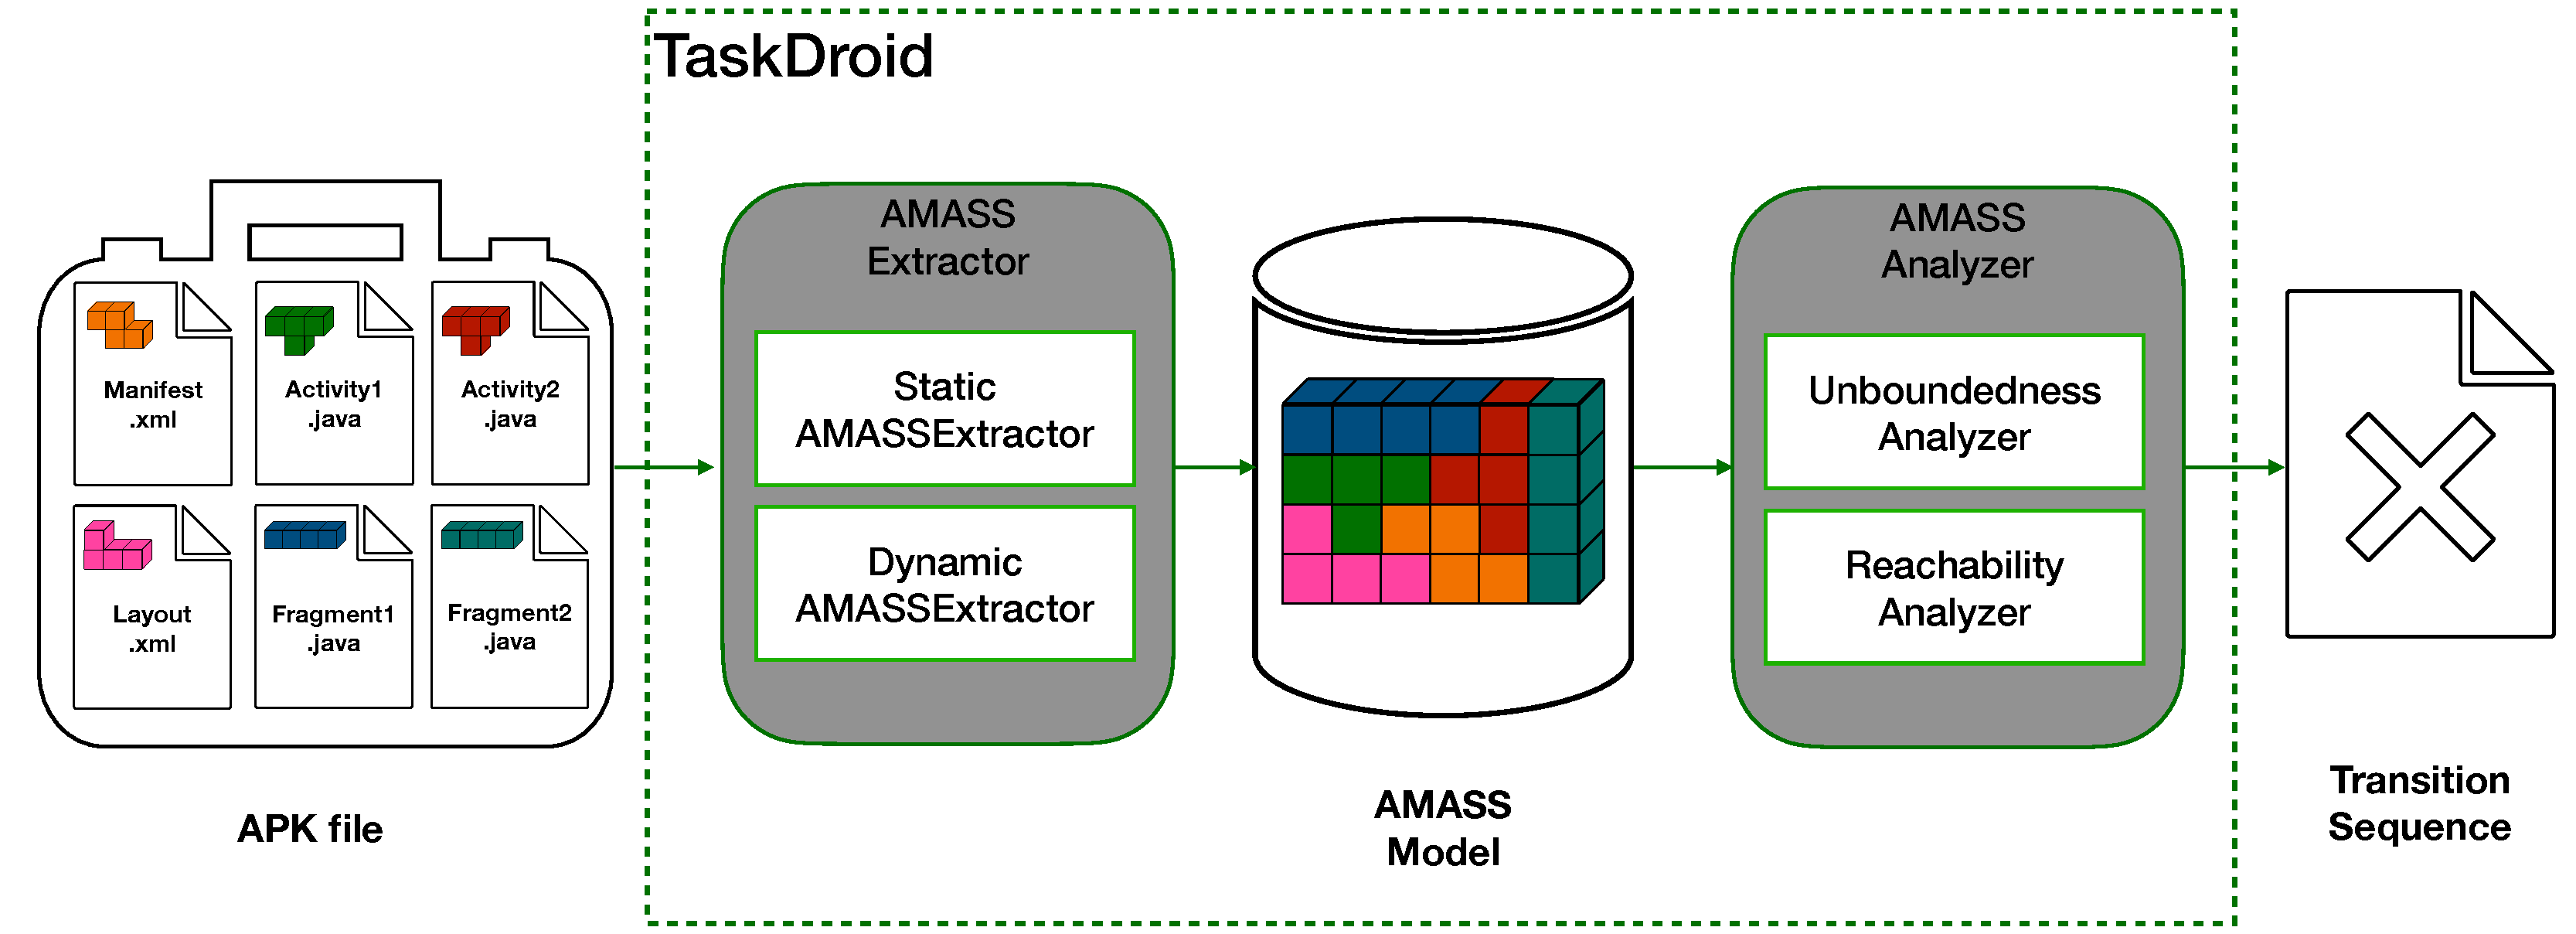
\includegraphics[scale=0.23]{taskdroid.pdf}
	\caption{Architecture of TaskDroid}
	\label{fig:taskdroid}
\end{figure}

%%%%%%%%%%%%%%%%%%%%%%%%%%%%%%%%%%%%%%%%%%%%%%%%%%%%%%%%%%%%%%%%%%%%%%

\subsection{Evaluation}\label{sec:bench}

We evaluate the efficiency and effectiveness of TaskDroid on 8,887 open source and commercial apps 
(cf.\ Section~\ref{sec:scal} and Section~\ref{sec:manual}). 
Moreover, we evaluate the impact of different model extractors on the detection of task/fragment container unboundedness problems of these apps (Section~\ref{sec:cmp}).  

The benchmark used for the evaluation consists of 8,887 Android apps collected from Androzoo\footnote{\url{https://androzoo.uni.lu/}} which include all the 3,867 open-source apps in the F-Droid repository,\footnote{\url{https://f-droid.org/}} as well as 5,020 commercial apps in the Google Play market. 
For Google Play, the apps are selected according to the popularity (number of downloads).  
Statistics of these apps can be found in Table~\ref{tab:stat}.
%
%The average/maximum size of F-Droid apps are 4.9MB/285.0MB respectively, while the average/maximum size of Google Play apps are 15.7MB/361.9MB respectively (see Table~\ref{tab:stat}). 

\begin{table}[htbp]   
\begin{center}   
\begin{tabular}{|c|c|c|c|}   
    \hline   \textbf{Source} & \textbf{\# apps}  &{\begin{tabular}{c} \textbf{Avg/Max. size} \\\textbf{of apps}\end{tabular}} & {\bf \begin{tabular}{c} \# extracted models \\
    (static/dynamic)\end{tabular} }  \\   
    \hline   F-Droid & 3,867  &4.9M/285.0M  & 3,471 (2,580/891)  \\ 
    \hline   Google Play & 5,020 &15.7M/361.9M  &4,612 (3,808/804)   \\  
\hline   
\end{tabular}  
\caption{Statistics of benchmarks \label{tab:stat}}   
\end{center}   
\end{table}

{\sf AMASSExtractor} extracts {\AMASS} models from the APK files as described in Section~\ref{sec:apk2amass}. 
\begin{itemize}
\item Out of the 3,867 F-Droid (resp.\ 5,020 Google Play) apps, static {\sf AMASSExtractor} extracts 2,580 (resp.\ 3,808) {\AMASS} models. Static {\sf AMASSExtractor} fails on 1,287 F-Droid (resp. 1,212 Google Play) apps, which is attributed to the fact that Soot fails to decompile the APK files or the source codes of the apps are obfuscated or encrypted. 

\item Out of the 2,580 models that are extracted from the F-Droid apps (called F-Droid models for short) by static {\sf AMASSExtractor} and 3,808 models that are extracted from the Google Play apps  (called Google-Play models for short) by static {\sf AMASSExtractor}, ICCBot$_{\AMASS}$ discovers that 311 F-Droid models and 501 Google-Play models respectively involve cross-app ICCs. 
Note that although ICCBot$_{\AMASS}$ discovers that these models involve cross-app ICCs, each of these models is extracted from \emph{one} APK file and the cross-app ICCs therein have not been dealt with yet. 
To remedy this, we tried to manually identify the APK files involved in these cross-app ICCs by searching for their package names. In the end, for 125 F-Droid apps and 211 Google-Play apps respectively, we provided the missing APK files involved in the cross-app ICCs of these apps and successfully constructed the {\AMASS} models for them where the cross-app ICCs are modeled. The average/maximum numbers and sizes of these missing apps involved in cross-app ICCs as well as the sizes of the extracted models are shown in Table~\ref{tab:missing-app}. Afterwards, these models can be analyzed in the same way as a model that is extracted from one APK file.
%
\item Moreover, among the 1,287 F-Droid (resp.\ 1,212 Google Play) apps that cannot be decompiled, dynamic {\sf AMASS} extracts 891 (resp.\ 804) {\AMASS} models. Dynamic {\sf AMASSExtractor} fails on 396 F-Droid (resp.\ 408 Google Play) apps, which is attributed to the fact that some apps cannot be launched, or crash after launching, or require user name and password to proceed after launching.  
\end{itemize}


\begin{table}
\begin{center}   
\begin{tabular}{|c | c | c |c |c |c |c |c |c |c |}   
    \hline    
    \multirow{2}{*}{\textbf{Source}}   & {\bf \begin{tabular}{c} \#apps containing \\ cross-app ICCs \end{tabular}} & {\begin{tabular}{c} \textbf{avg/max. numbers} \\ \textbf{of  missing apps}\end{tabular}}  & \begin{tabular}{c} \textbf{avg/max. sizes}  \\ {\bf of missing apps} \end{tabular}  & \multicolumn{3}{c|}{\textbf{avg/max. sizes of models}}  \\   
    \cline{5-7}    
    &&& & $|\act|$& $|\frag|$ & $|\Delta|$    \\ 
    \hline   
    F-Droid& 125 & 1.2/2 & 6.8M/103.2M& 6.2/38& 0.9/11 & 10.1/66   \\ 
    \hline   
    Google Play&804 & 1.5/2 &16.1M/153.3M& 7.9/19&1.1/20&14.5/97   \\  
\hline   
\end{tabular}   
\caption{Statistics of the missing apps involved in cross-app ICCs}
 \label{tab:missing-app} 
\end{center}   
\end{table}




\subsubsection{The efficiency of {\tool}}\label{sec:scal}
We investigate the efficiency and scalability of {\tool} by examining all 3,471 F-Droid and 4,612 Google Play apps for which AMASS models are extracted. For each app, static {\sf AMASSExtractor} extracts an {\AMASS} model from the APK file statically, where the timeout is set to 300 seconds. 
Moreover, for the apps where static {\sf AMASSExtractor} fails, dynamic {\sf AMASSExtractor} extracts an {\AMASS} model dynamically, where the time out is set to 600 seconds. 
The average/maximum sizes of the extracted models as well as the extraction time are shown in Table~\ref{tab:amass}--\ref{tab:amassdyn}.

%From Table~\ref{tab:amass},
It can be observed that, for the statically extracted models, the average/maximum size (number of transition rules, activities, fragments) of F-Droid apps is much smaller than that of Google Play apps. This is expected, since the  Google Play apps are considerably more complex than F-Droid open-source apps.
Moreover, the average time spent in the static model extraction of Google Play apps is over 5 times more than that of F-Droid apps.
Similar phenomenon happens for the dynamic model extraction, though the difference is slightly smaller. 
%than the static model extraction. 

%From Table~\ref{tab:amass}, 
Furthermore, static {\sf AMASSExtractor} can extract the {\sf AMASS} models for F-Droid apps in less than 1 minute and for Google Play apps in less than 4 mins, whereas %. On the other hand, from Table~\ref{tab:amassdyn}, 
dynamic {\sf AMASSExtractor} can extract the {\sf AMASS} models for F-Droid apps in around 5 mins and for Google Play apps in around 10 mins. The static model extraction is faster than the dynamic one, while the dynamic approach can deal with the apps that the static approach fails.

%Similarly, for the dynamic model extraction,  the average/maximum size (number of transition rules, activities, fragments) of F-Droid apps is much smaller than that of Google Play apps

%of transition rules ($|\Delta|$) is 7.9 (resp. 21.0) for F-Droid (resp. GooglePlay), the average number of activities ($|\act|$) is 4.9 (resp. 7.1) for F-Droid (resp. GooglePlay), the average number of fragments ($|\frag|$) is 0.5 (resp. 1.0) for F-Droid (resp. GooglePlay),
%the maximum number of transition rules ($|\Delta|$) for the AMASS models is 475 (resp. 1956) for F-Droid (resp. GooglePlay), the average number of activities ($|\act|$) is 70 (resp. 509) for F-Droid (resp. GooglePlay), the average number of fragments ($|\frag|$) is 16 (resp. 121) for F-Droid (resp. GooglePlay).
%The column Time shows the time used to extract the model. In general, the apps from Google Play are considerably more complex than F-Droid open-source apps, which incur about 6 times more processing time and 5 times more transition rules number.

\begin{table}[htbp]   
\begin{center}   
\begin{tabular}{|c |c |c |c |c |c |c |c|}   
    \hline    
    \multirow{2}{*}{\textbf{Source}}   &\multicolumn{3}{c|}{\textbf{Avg/Max. size of models}} & \multirow{2}{*}{\textbf{Avg. Time}} \\   
    \cline{2-4}    
    & $|\act|$& $|\frag|$ & $|\Delta|$ &   \\ 
    \hline   
    F-Droid & 4.9/70& 0.5/16 & 7.9/475 &  43.5s  \\ 
    \hline   
    Google Play & 7.1/509&1.0/121&21.0/1,956 & 234.6s  \\  
\hline   
\end{tabular}   
\caption{Static AMASSExtractor \label{tab:amass} }
\end{center}   
\begin{center}   
\begin{tabular}{|c|c|c|c|c|c|c|}   
    \hline  \multirow{2}{*}{\textbf{Source}}  &\multicolumn{2}{c|}{\textbf{Avg/Max. size of \AMASS}} & \multirow{2}{*}{\textbf{Avg. Time}} \\   
    \cline{2-3}   & $|\act|$& $|\Delta|$ &   \\ 
    \hline   F-Droid & 6.1/31&15.3/71 & 313.4s  \\  
    \hline   Google Play & 11.2/43&28.1/129 & 593.2s  \\  
\hline   
\end{tabular}   
\caption{Dynamic AMASSExtractor \label{tab:amassdyn} }
\end{center}   
\end{table}


%For each app in our bench marck (resp. 25 popular apps selected randomly from GooglePlay with more than 100,000 downloads), we build up an AMASS model from APK files via static extractor (resp. dynamic extractor), where the timeout is set to 300 seconds. The experimental results are shown in Table~\ref{tab:amass} (resp. Table~\ref{tab:amassdyn}),

%%%%%%%%%%%%%%%%%%%%%%%%%%%%%%%%%%%%%%%%%%%%%%%%%%%%%%%%%%%%%%%%%%%%%%%%%%%



%We investigate the effectiveness of our analysis approach in 
To detect %apps exhibiting the 
task/fragment container unboundedness vulnerabilities, the timeout is set to 30 seconds, the height $\hbar$ of tasks is set to 6 and $k$ (i.e., the number of interplaying tasks, cf.\ Section~\ref{sec:static}) is set to 2.

We first consider \revision{Android 13.0}. The results of task unboundedness (resp.\ fragment container unboundedness) 
are presented in Table~\ref{tab:taskbound}--\ref{tab:frgbound}. 
%Column \# Unbounded apps shows the number of detected apps which suffer from task unboundedness (resp. fragment stack unboundedness). Column \# Faulty cycles per app shows the number of witness cycles of each task unbounded (resp. fragment stack unbounded) app. Column Time shows the average time to perform the analysis. 
As one may see, {\tool} is highly efficient %fast 
in analyzing the {\AMASS} models, % against the task and fragment container unboundedness problems, 
which can be done 
in less than 0.1 seconds per app on average.
%
Moreover, {\tool} identifies 485 (14.0\%) F-Droid and 559 (12.1\%) GooglePlay models as ``task unbounded''.
On the other hand, %from Table~\ref{tab:frgbound}, 
{\tool} identifies 193 (5.6\%) F-Droid  and  293 (6.4\%) Google Play models as ``fragment container unbounded''. 
Finally, the number of witness cycles discovered for the unbounded models is around 3 per app on average.

\begin{table}[htbp]   
\begin{center}   
\begin{tabular}{|c|c|c|c|}   
    \hline   \textbf{Source}  &\begin{tabular}{c}\textbf{\#Unbounded}\\ \textbf{models}\end{tabular} & \begin{tabular}{c} \#\textbf{witness cycles} \\ \textbf{per model}\end{tabular} & \textbf{Time(s)} \\   
    \hline   F-Droid & 485/3,471 (14.0\%) & 3.3 &  0.05s  \\ 
    % \hline   F-Droid & Activity-based &413/3,471(11.9\%) & 3.1 &  0.05s  \\ 
    \hline   Google Play & 559/4,612 (12.1\%)&3.9 & 0.1s  \\  
    % \hline   Google Play & Activity-based &468/4,612(10.1\%)&3.4 & 0.1s  \\  
    %\hline   Google Play\# &9(36\%)&4.2 & 10.3s  \\  
\hline   
\end{tabular}   
\caption{Task Unboundedness \label{tab:taskbound} }
\end{center}   
\end{table}

\begin{table}[htbp]   
\begin{center}   
\begin{tabular}{|c|c|c|c|}   
    \hline   \textbf{Source} &\begin{tabular}{c}\textbf{\#Unbounded}\\ \textbf{models}\end{tabular} & \begin{tabular}{c} \#\textbf{witness cycles} \\ \textbf{per model}\end{tabular} & \textbf{Time(s)} \\   
    \hline   F-Droid & 193/2,580 (7.5\%) & 2.5 &  0.05   \\ 
    \hline   Google Play &293/3,808 (7.7\%)&3.0 & 0.1   \\  
\hline   
\end{tabular}   
\caption{Fragment Container Unboundedness \label{tab:frgbound} }
\end{center}   
\end{table}

We then consider Android 6.0--12.0 and compare the results for these versions with those for \revision{Android 13.0}. As shown in Figure~\ref{fig:cmp-and}, the numbers of task unbounded F-Droid (resp.\ Google Play) apps are slightly different for different versions, while the numbers of fragment container unbounded F-Droid (resp.\ Google Play) apps are the same for different versions. This phenomenon is explained by that the semantics of $\AOAMASS$ is slightly different across Android versions, while the semantics of $\FOAMASS$ is the same for all these versions. To have a closer look, we can see that the numbers of task unbounded F-Droid (resp.\ Google Play) apps for Android 7.0, Android 8.0--10.0, and \revision{Android 11.0--13.0} are close to each other, and are slightly away from that of Android 6.0. This is explained by that Android 6.0 uses a different task allocation mechanism from the others. 


%%%%%%%%%%%%%%%%%%%%%%%%%%
%%%%%%%%%%%%%%%%%%%%%%%%%%
\hide{
\revision{Although our algorithm is primarily designed for analyzing individual apps, it can also handle the analysis of interactions between multiple apps. In such cases, we construct an {\AMASS} model that includes the activities, fragments, transition rules, and other components of the relevant apps. The main activity of the analyzed app is set as the main activity $A_0$ of the model. In the sequel, these apps can be treated as one app for further analysis. There are $311$ (resp. $501$) models comprising the cross-app ICC out of $3,471$ (resp. $4,612$) extracted models in F-Droid (resp. Google Play).  As illustrated in Figure~\ref{fig:cross-app}, when considering cross-app ICC, we obtain the same results in detecting fragment container unboundedness vulnerabilities, as app-switching does not add new activities to the analyzed app.  Additionally, there is a slight increase in the detection of task unbounded apps. 
This is primarily due to the fact that over 91\% of the models (739 out of 812) with cross-app ICC exhibit the behavior of remaining in the background after switching to another app, which is similar to the situation when cross-app ICC is not considered.}
}
%%%%%%%%%%%%%%%%%%%%%%%%%%
%%%%%%%%%%%%%%%%%%%%%%%%%%

% the number of the fragment container unbounded models detected is the same under Android 6.0-Android 12.0, the number of the task unbounded models detected under Android 6.0, Android 8.0-Android 10.0 is more than the one under Android 12.0, while the number of the task unbounded models detected under Android 7.0 is less than the one under Android 12.0.

%In summary, for 3,471 F-Droid (resp. 4,612 Google Play)  apps, TaskDroid can extract the {\AMASS} models from APK files and finish the unboundedness analysis in around 5 minutes (resp. 10 minutes) per app, where the vast majority of the time is spent in the extraction of an {\AMASS} model and the unboundedness analysis of the model is pretty fast. 

%It can be observed that, for apps from F-Droid, when we adopt a simple $\AMASS$ model, 108 (out of 2,580) apps are found to have UBA abnormality, but when a full $\AMASS$ model is used, 251 apps are detected, which gives an increase of 132\%. The same thing is observed for the apps from Google Play. The increases on the number of abnormal transition rules are even higher. This highlights the importance and benefit of adopting a full-fledged semantics for the multitasking mechanism, including features such as fragments. We remark that a full  $\AMASS$ model allows to capture  more cases of UBA, for instance, the case (1) with $\ntkflag$ and the case (2) where fragments are involved. 
%In terms of the efficiency, the average time is 0.2 second for relatively small apps from F-Droid and 1.1 second for larger apps from Google Play. 





% \begin{figure}%[h]
% \centering
% 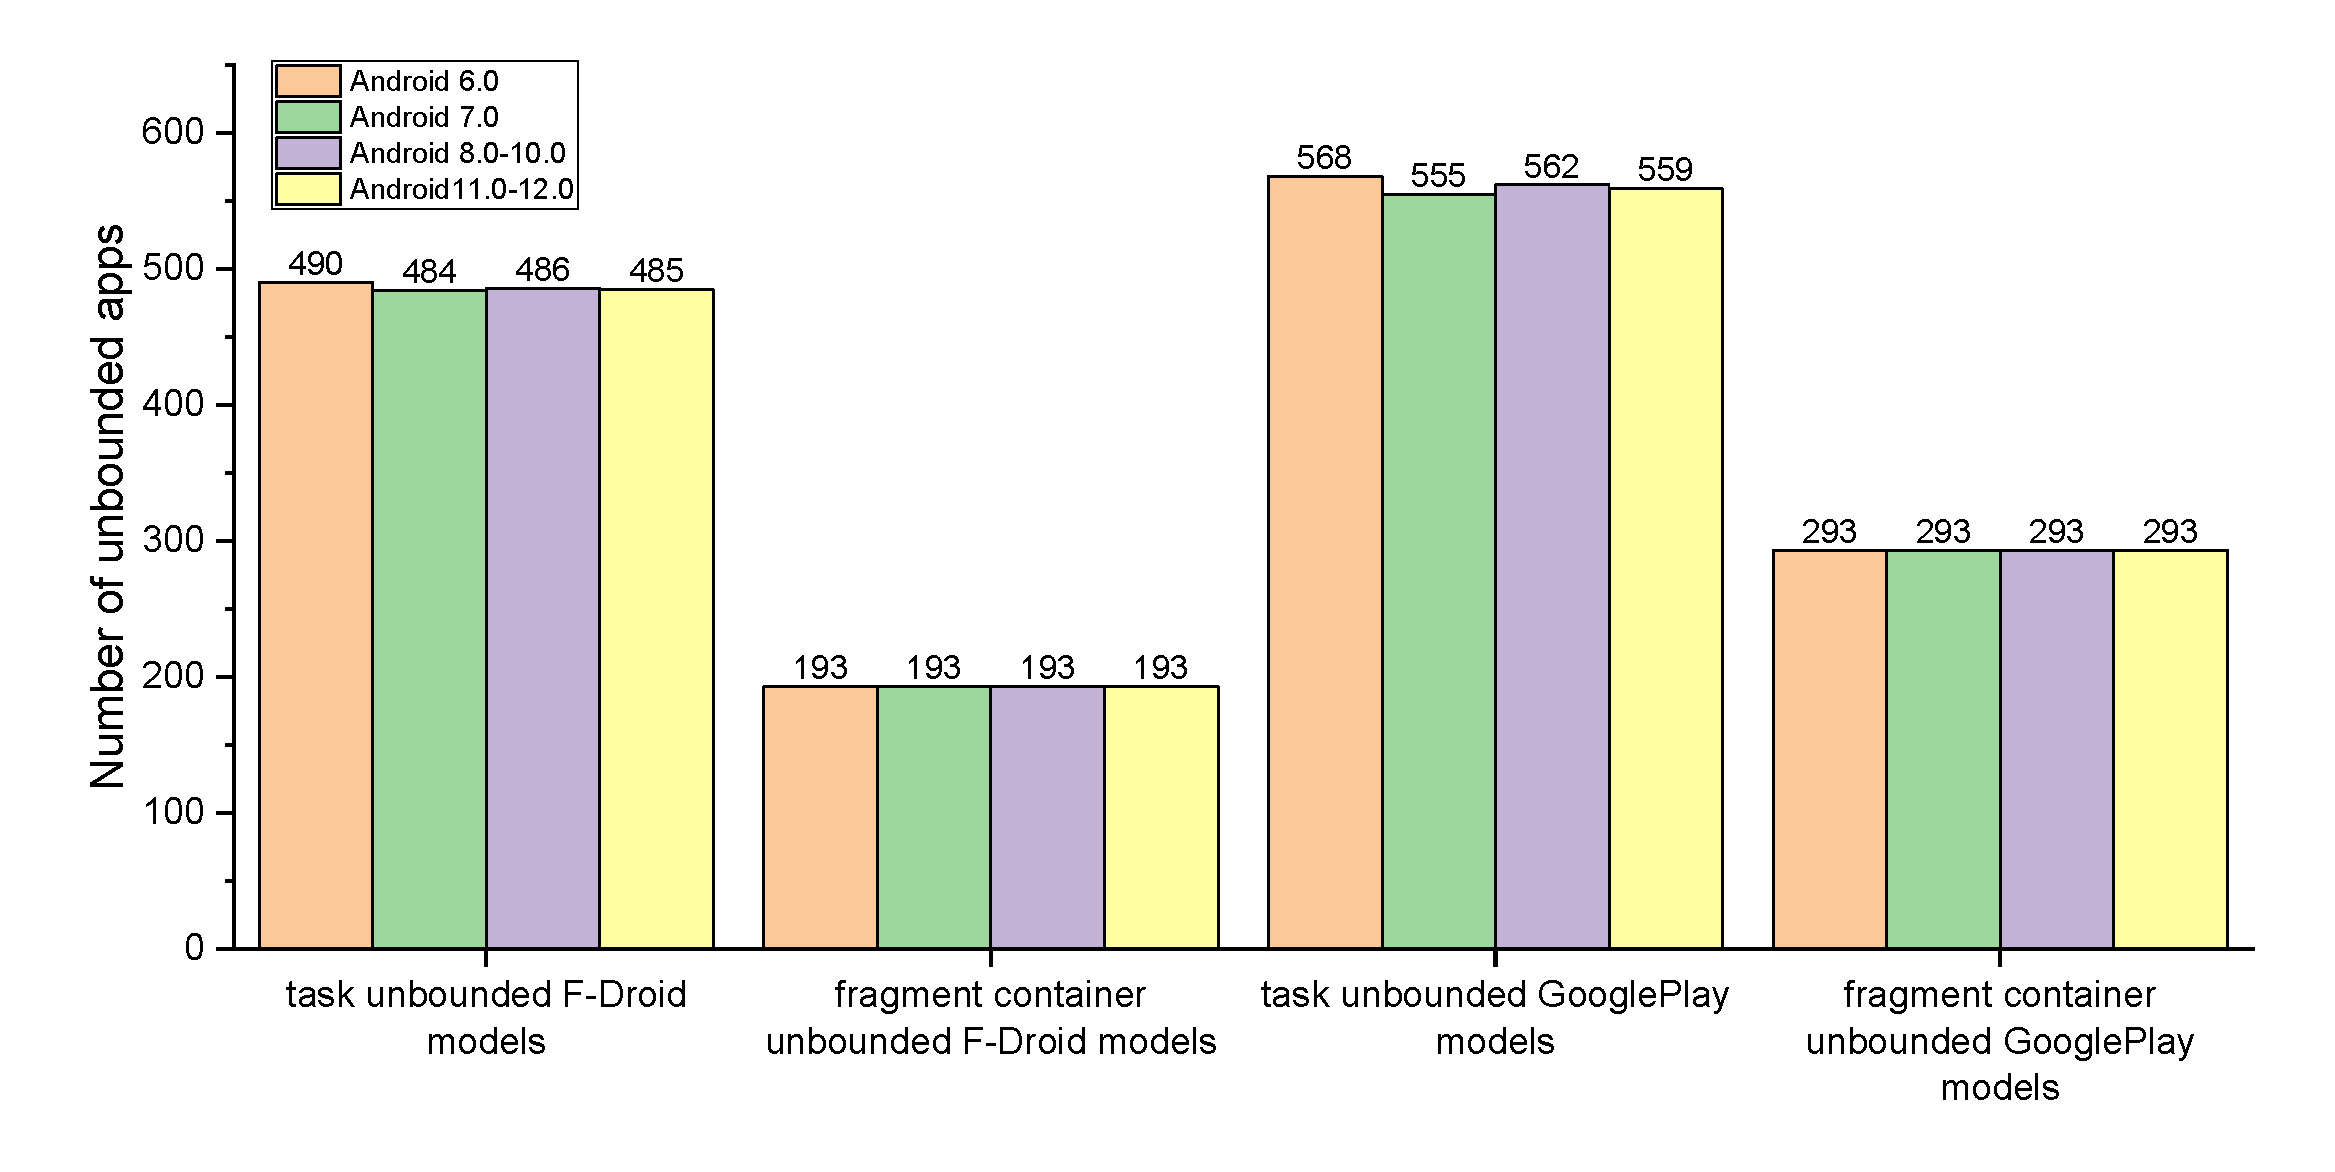
\includegraphics[scale=0.35]{android-version.pdf}
% \caption{Unboundedness under different Android versions}
% \label{fig:ubd-android}
% \end{figure}
\begin{figure}[htbp]
	\begin{minipage}[t]{0.49\linewidth}
		\centering
		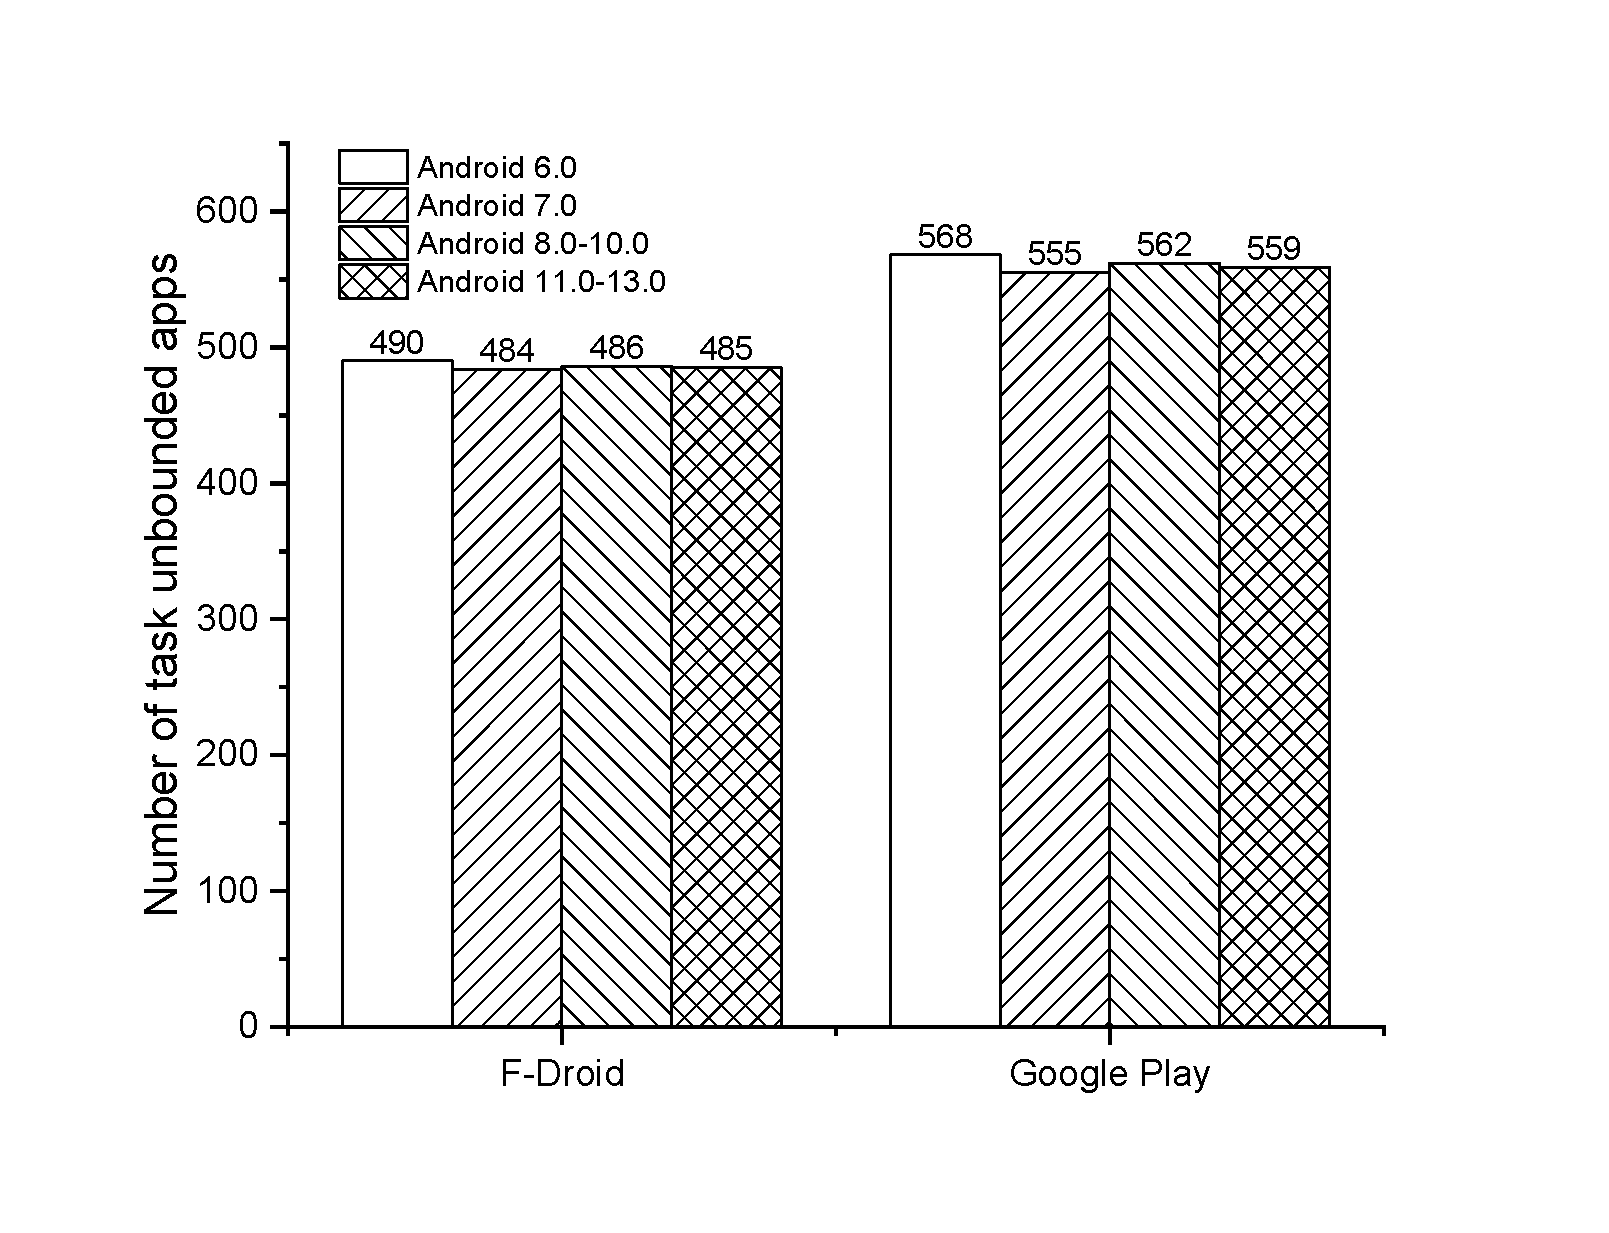
\includegraphics[width=3.2in]{cmp-and-task.pdf}
	\end{minipage}
	\begin{minipage}[t]{0.49\linewidth}
		\centering
		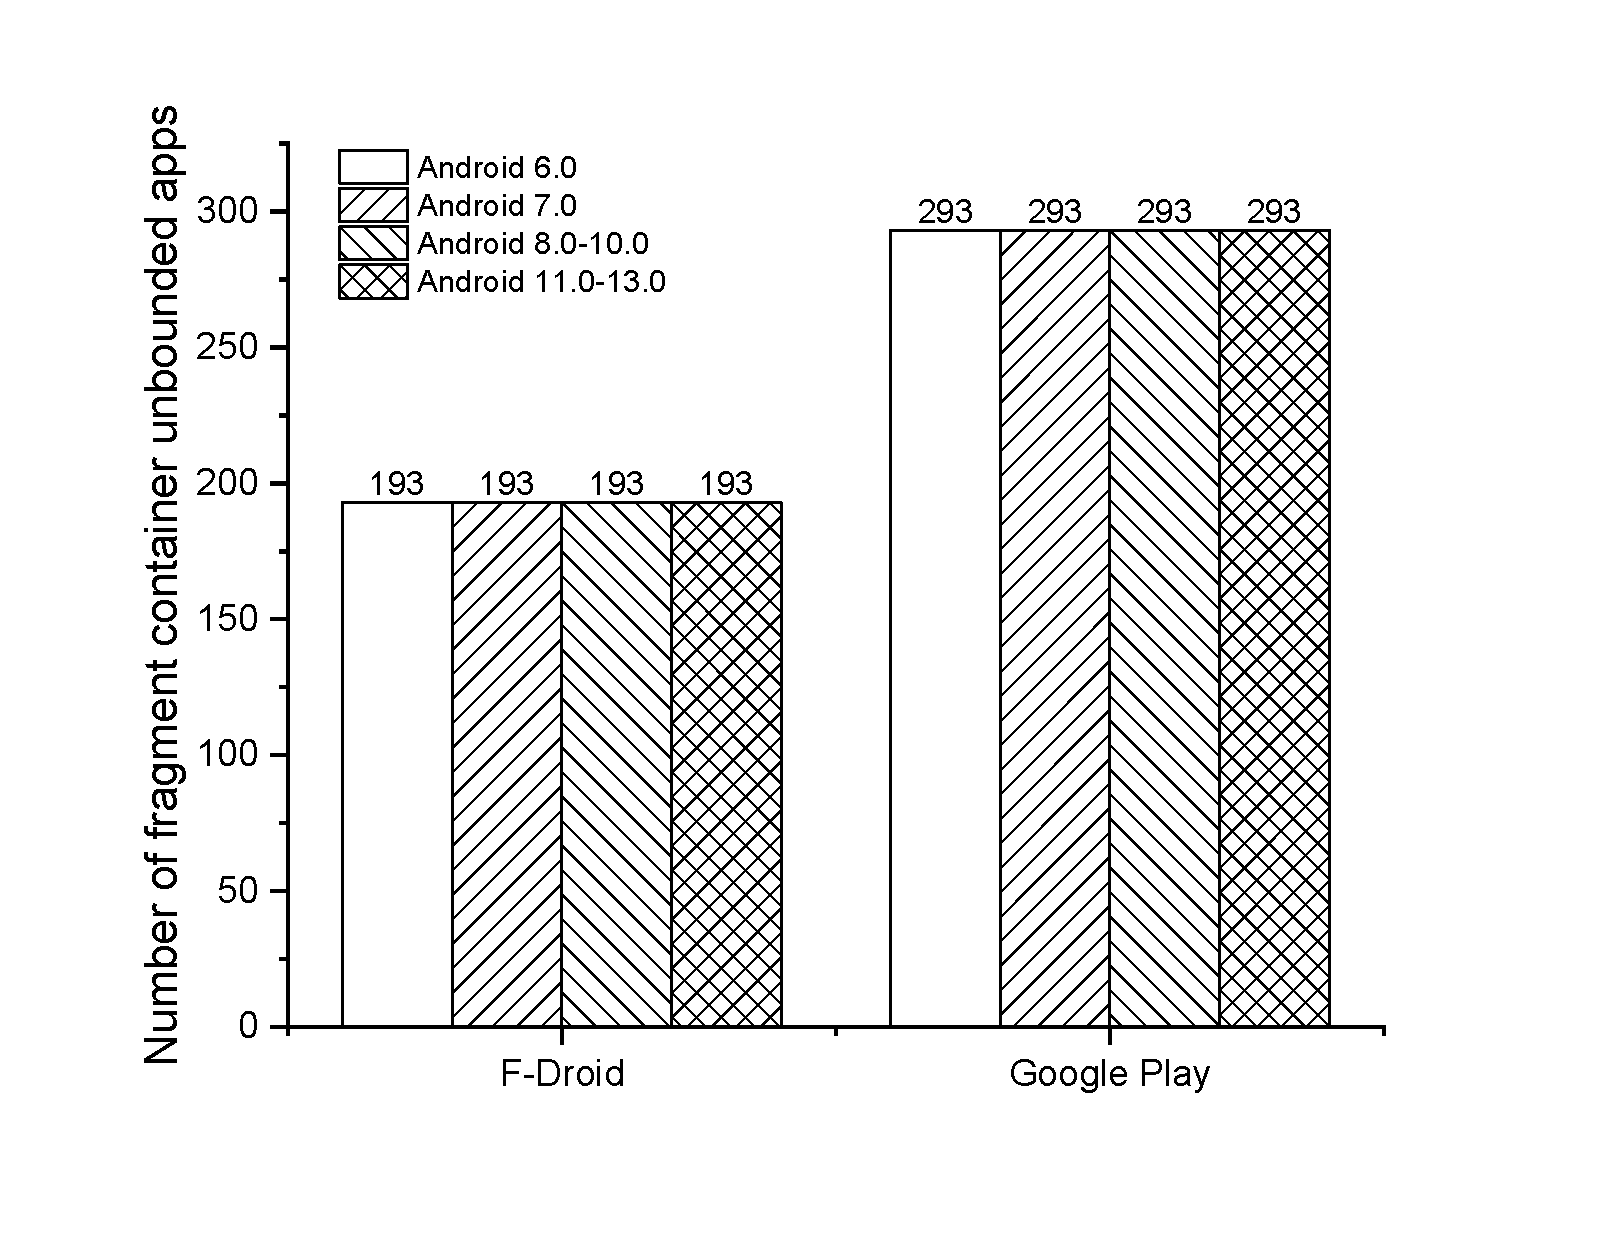
\includegraphics[width=3.2in]{cmp-and-frag.pdf}
	\end{minipage}
	\caption{\revision{Comparison of the results for different Android versions}}
	\label{fig:cmp-and}
\end{figure}

\hide{
\begin{figure}
	\begin{minipage}[t]{0.49\linewidth}
		\centering
		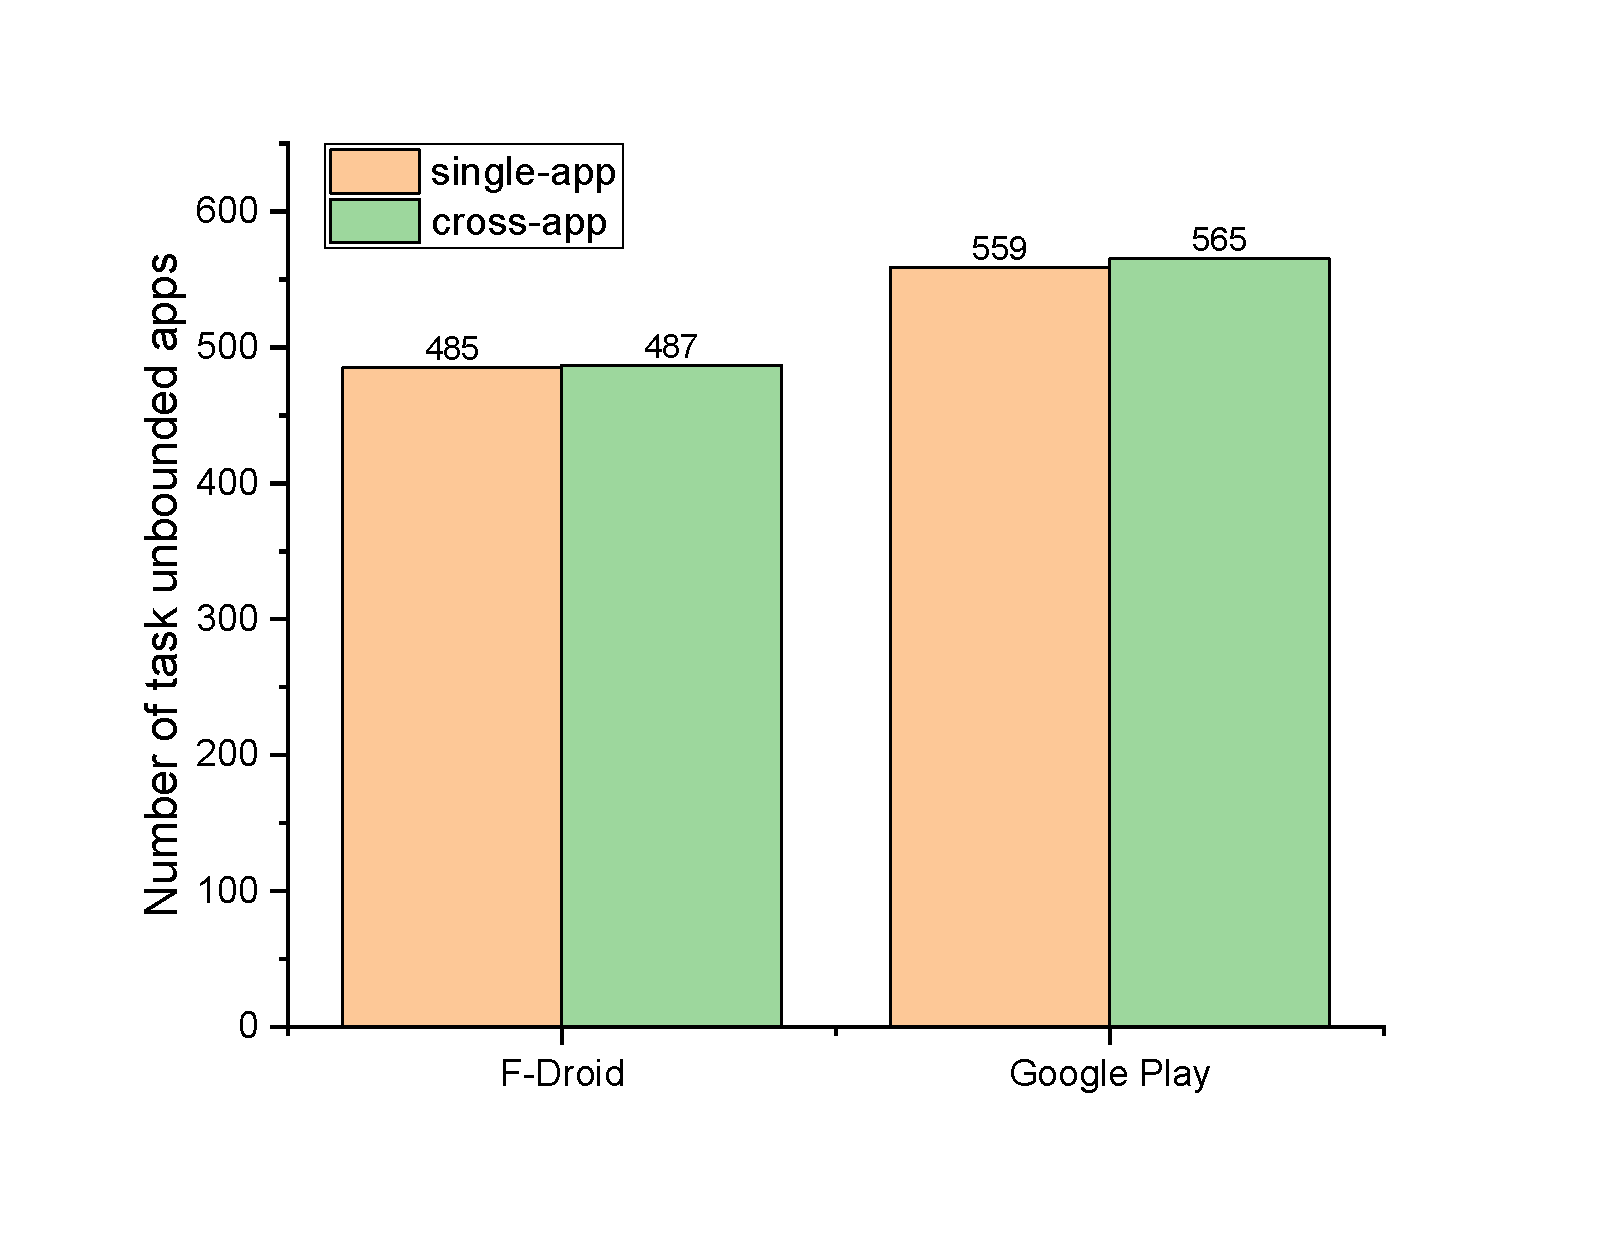
\includegraphics[width=3.2in]{task_unb_cross.pdf}
	\end{minipage}
	\begin{minipage}[t]{0.49\linewidth}
		\centering
		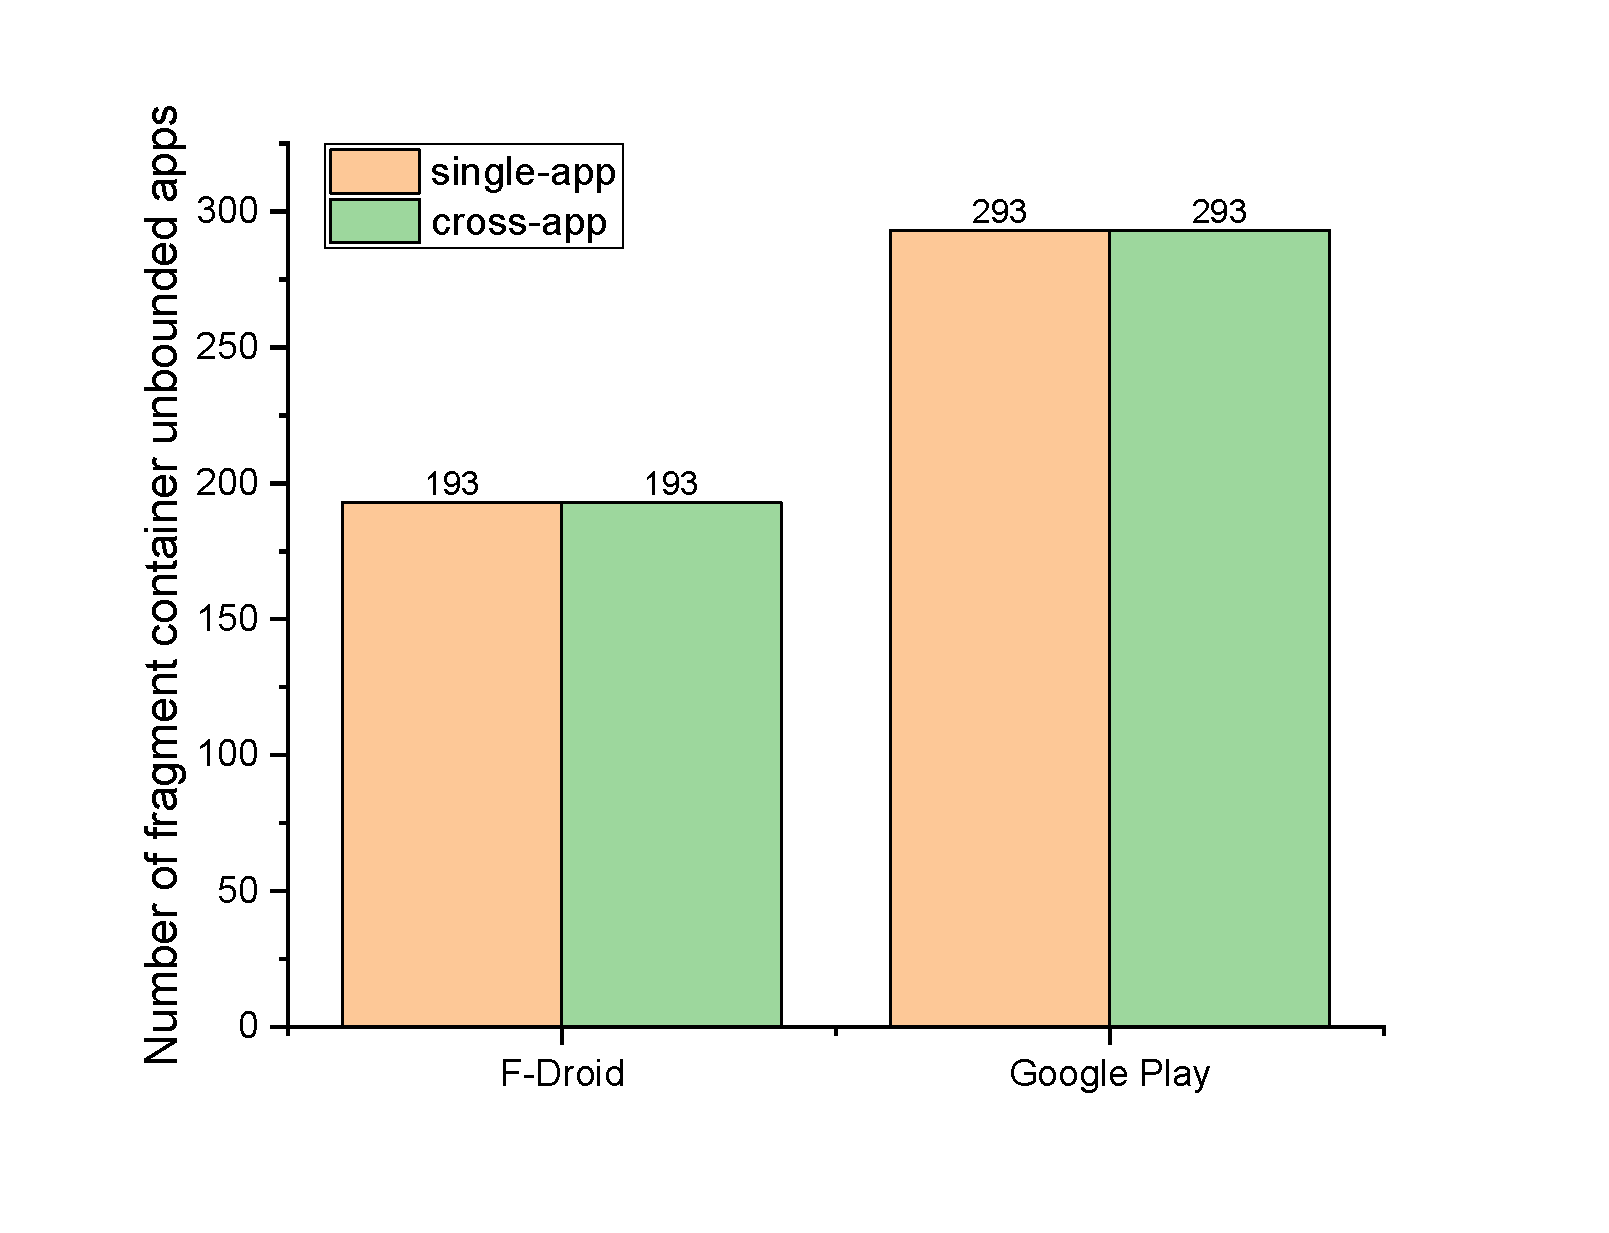
\includegraphics[width=3.2in]{frag_unb_cross.pdf}
	\end{minipage}
	\caption{Unboundedness when (resp. not) considering cross-app ICC}
	\label{fig:cross-app}
\end{figure}
}



\subsubsection{The effectiveness of \tool} \label{sec:manual}
 %
We investigate whether {\tool} can accurately detect task/fragment container unboundedness vulnerabilities, and the abnormal behavior caused by these vulnerabilities in Android mobile device.  
To this end, we randomly select 50 apps from those that are identified as ``task unbounded'' and  ``fragment container unbounded'' by {\tool} respectively, in each case 25 are from F-Droid and 25 are from GooglePlay.
The information of these apps can be found in  Appendix~\ref{app:table}, Table~\ref{tab:t-unb-rand-fd}~--~\ref{tab:fc-unb-rand-gg}. 


%\begin{table*}[t]
%\begin{center}   
%\caption{Statistics of 50 randomly selected ``task-unbounded'' apps \label{tab:t-unb-rand} }
%\begin{tabular}{|c|c|c|c|c|c|}   
%    \hline   \textbf{Source} &\textbf{Package name} &\textbf{$|\act|$} & \textbf{$|\frag|$} & \textbf{$|\Delta|$} & \textbf{Size(MB)} \\   
%%
%    \hline   F-Droid  & org.gnucash.android & 10 & 2& 32 & 2.71  \\ 
%    \hline   F-Droid  & systems.byteswap.aiproute & 3& 0& 3& 1.08  \\ 
%    \hline   F-Droid  & max.music\_cyclon & 2& 0& 2& 1.81 \\ 
%    \hline   F-Droid  & com.matburt.mobileorg & 8& 0& 9& 1.36 \\ 
%    \hline   F-Droid  & org.npr.android.news & 5& 0& 8& 0.92 \\ 
%    \hline   F-Droid  & com.commonsware.android.arXiv & 8& 0& 12& 0.52 \\ 
%    \hline   F-Droid  & net.mabako.steamgifts & 6& 1& 24& 2.66 \\ 
%    \hline   F-Droid  & com.app.Zensuren & 17& 0& 22& 0.17 \\ 
%    \hline   F-Droid  & uk.co.busydoingnothing.prevo & 4& 0& 5& 11.79 \\ 
%    \hline   F-Droid  & de.drhoffmannsoftware.calcvac & 14& 0& 24& 0.9 \\ 
%    \hline   F-Droid  & org.sasehash.burgerwp & 2& 0& 3& 1.76 \\ 
%    \hline   F-Droid  & com.mikifus.padland & 6& 1& 18& 1.07  \\ 
%    \hline   F-Droid  & org.evilsoft.pathfinder.reference & 5& 0& 8& 22.02  \\ 
%    \hline   F-Droid  & com.android.keepass & 4& 0& 6& 1.65  \\ 
%    \hline   F-Droid  & de.bloosberg.basti.childresuscalc & 2& 0& 2& 1.41  \\ 
%    \hline   F-Droid  & com.samebits.beacon.locator & 2& 0& 2& 1.98  \\ 
%    \hline   F-Droid  & ohm.quickdice & 9& 0& 14& 1.41  \\ 
%    \hline   F-Droid  & org.saiditnet.redreader & 11& 1& 51& 4.99  \\ 
%    \hline   F-Droid  & com.gianlu.aria2app & 13& 0& 31& 21.11  \\ 
%    \hline   F-Droid  & net.artificialworlds.rabbitescape & 3& 0& 3& 18.81  \\ 
%    \hline   F-Droid  & com.sam.hex & 10& 0& 23& 0.76  \\ 
%    \hline   F-Droid  & com.kaliturin.blacklist & 2& 0& 2& 2.06  \\ 
%    \hline   F-Droid  & de.schildbach.oeffi & 10& 0& 35& 1.79  \\ 
%    \hline   F-Droid  & com.aurora.store & 22& 0& 56& 5.47  \\ 
%    \hline   F-Droid  & com.adrienpoupa.attestationcoronavirus & 2& 0& 2& 3.58  \\ 
%%    \hline   \multicolumn{2}{|c|}{\textbf{Average}} & 7.2& 0.2& 15.9& 4.6  \\ 
%%
%    \hline   GooglePlay  & com.abdulqawi.ali.mosabqa & 8& 0& 25& 2.84  \\ 
%    \hline   GooglePlay  & com.music.star.player & 3& 3& 25& 2.38  \\ 
%    \hline   GooglePlay  & com.drclabs.android.wootchecker & 11& 0& 18& 0.84  \\ 
%    \hline   GooglePlay  & com.hotels.hotelsmecca & 6& 1& 16& 16.43  \\ 
%    \hline   GooglePlay  & com.airg.hookt & 6& 0& 12& 10.59  \\ 
%    \hline   GooglePlay  & com.holidu.holidu & 2& 0& 2& 4.04  \\ 
%    \hline   GooglePlay  & com.appkey.english3000freekata & 28& 0& 97& 1.06  \\ 
%    \hline   GooglePlay  & socials.com.application & 34& 0& 122& 3.75  \\ 
%    \hline   GooglePlay  & www.genting.rwgenting & 3& 0& 5& 12.78  \\ 
%    \hline   GooglePlay  & com.goldenhammer.beisboldominicana & 3& 1& 10& 4.58  \\ 
%    \hline   GooglePlay  & com.travolution.seoultravelpass & 5& 0& 10& 4.58  \\ 
%    \hline   GooglePlay  & com.ic.myMoneyTracker & 25& 0& 60& 3.39  \\ 
%    \hline   GooglePlay  & tekcarem.gebeliktakibi & 59& 0& 255& 3.15  \\ 
%    \hline   GooglePlay  & de.fckoeln.app & 22& 0& 45& 40.77  \\ 
%    \hline   GooglePlay  & de.twokit.castbrowser & 5& 0& 8& 3.79  \\ 
%    \hline   GooglePlay  & com.TWTD.FLIXMOVIE & 6& 0& 10& 7.73  \\ 
%    \hline   GooglePlay  & com.emeint.android.mwallet.tub & 10& 0& 95& 59.02  \\ 
%    \hline   GooglePlay  & com.ctt.celltrak2 & 22& 0& 80& 11.31  \\ 
%    \hline   GooglePlay  & biz.mobinex.android.apps.cep\_sifrematik & 11& 0& 34& 3.54  \\ 
%    \hline   GooglePlay  & com.linesmarts.linesmartsfree & 4& 0& 4& 28.47  \\ 
%    \hline   GooglePlay  & com.nhiApp.v1 & 8& 9& 107& 26.6  \\ 
%    \hline   GooglePlay  & com.alfarooqislamicresearchcenter & 34& 0& 78& 13.83  \\ 
%    \hline   GooglePlay  & com.objectremover.touchretouch & 14& 0& 19& 11.28  \\ 
%    \hline   GooglePlay  & com.vwfs.phototan & 3& 0& 5& 27.23  \\ 
%    \hline   GooglePlay  & com.sg.apphelperstore & 5& 0& 6& 6.56  \\ 
%%    \hline   \multicolumn{2}{|c|}{\textbf{Average}} & 13.5& 0.6& 45.9& 12.4  \\ 
%
%    
%\hline   
%\end{tabular}   
%\end{center}   
%\end{table*}
%
%\begin{table*}[t]
%\begin{center}   
%\caption{Statistics of 50 randomly selected ``fragment-container unbounded'' apps \label{tab:fc-unb-rand} }
%\begin{tabular}{|c|c|c|c|c|c|}   
%    \hline   \textbf{Source} &\textbf{Package name} &\textbf{$|\act|$} & \textbf{$|\frag|$} & \textbf{$|\Delta|$} & \textbf{Size(MB)} \\   
%%
%    \hline   F-Droid & org.ligi.fahrplan & 6& 5& 46& 1.83  \\ 
%    \hline   F-Droid  & io.gitlab.allenb1.todolist & 6& 3& 11& 1.05  \\ 
%    \hline   F-Droid  & naman14.timber & 5& 3& 15& 5.8  \\ 
%    \hline   F-Droid  & me.anon.grow & 4& 3& 30& 6.46  \\ 
%    \hline   F-Droid  & com.wikijourney.wikijourney & 1& 2& 7& 4.27  \\ 
%    \hline   F-Droid  & com.mattallen.loaned & 3& 1& 5& 1.01  \\ 
%    \hline   F-Droid  & com.ymber.eleven & 1& 2& 15& 10.38  \\ 
%    \hline   F-Droid  & com.syncedsynapse.kore2 &2& 1& 5& 2.22  \\ 
%    \hline   F-Droid  & net.momodalo.app.vimtouch & 5& 1& 9& 3.44  \\ 
%    \hline   F-Droid  & com.csipsimple & 12& 2& 22& 11.56  \\ 
%    \hline   F-Droid  & ch.corten.aha.worldclock & 4& 3& 13& 1.4  \\ 
%    \hline   F-Droid  & org.wikimedia.commons.wikimedia & 3& 6& 44& 15.0  \\ 
%    \hline   F-Droid  & com.llamacorp.equate & 1& 1& 3& 0.39  \\ 
%    \hline   F-Droid  & koeln.mop.elpeefpe & 4& 2& 11& 1.59  \\ 
%    \hline   F-Droid  & fr.kwiatkowski.ApkTrack & 1& 2& 13& 2.32  \\ 
%    \hline   F-Droid  & eu.siacs.conversations.legacy & 17& 2& 88& 11.12  \\ 
%    \hline   F-Droid  & com.artifex.mupdfdemo & 4& 2& 5& 25.68  \\ 
%    \hline   F-Droid  & org.osmdroid  & 15& 3& 28& 4.62  \\ 
%    \hline   F-Droid  & com.haha01haha01.harail & 4& 1& 6& 0.69   \\ 
%    \hline   F-Droid  & com.owncloud.android & 11& 4& 40& 3.8  \\ 
%    \hline   F-Droid  & org.cipherdyne.fwknop2 & 5& 2& 12& 2.63  \\ 
%    \hline   F-Droid  & edu.cmu.cylab.starslinger.demo & 4& 1& 8& 1.21  \\ 
%    \hline   F-Droid & com.commonslab.commonslab & 4& 6& 45& 14.72  \\ 
%    \hline   F-Droid  & hans.b.skewy1\_0 & 1& 6& 19& 6.45  \\ 
%    \hline   F-Droid  & com.twobuntu.twobuntu & 4& 3& 12& 0.75  \\ 
%%    \hline   \multicolumn{3}{|c|}{\textbf{Average}} & 5.1& 2.7& 20.5& 5.6  \\ 
%%
%    \hline   GooglePlay  & com.schoola2zlive & 11& 1& 40& 4.77  \\ 
%    \hline   GooglePlay  & com.endless.smoothierecipes & 3& 9& 110& 7.57  \\ 
%    \hline   GooglePlay  & com.traderumors & 5& 6& 28& 5.53  \\ 
%    \hline   GooglePlay & com.rakuten.room & 20& 19& 87& 20.1  \\ 
%    \hline   GooglePlay  & com.hotels.hotelsmecca & 6& 1& 16& 16.43  \\ 
%    \hline   GooglePlay  & br.com.prevapp03 & 34& 1& 80& 5.15  \\ 
%    \hline   GooglePlay  & com.star.mobile.video & 21& 1& 55& 7.98  \\ 
%    \hline   GooglePlay  & fr.elol.yams & 4& 6& 93& 8.75  \\ 
%    \hline   GooglePlay  & music.symphony.com.materialmusicv2 & 7& 3& 14& 3.39  \\ 
%    \hline   GooglePlay  & ru.sports.rfpl & 6& 1& 9& 8.33  \\ 
%    \hline   GooglePlay  & com.discsoft.daemonsync & 7& 1& 10& 10.06  \\ 
%    \hline   GooglePlay  & com.accuvally.android.accupass & 8& 1& 21& 11.62  \\ 
%    \hline   GooglePlay  & com.directv.navigator & 10& 7& 68& 41.66  \\ 
%    \hline   GooglePlay  & com.ldf.gulli.view & 13& 8& 49& 15.62  \\ 
%    \hline   GooglePlay  & kvp.jjy.MispAndroid320 & 14& 6& 51& 31.34  \\ 
%    \hline   GooglePlay  & de.wirfahrlehrer.easytheory & 3& 12& 144& 3.6  \\ 
%    \hline   GooglePlay  & com.mmb.mamitalk & 5& 4& 22& 8.19  \\ 
%    \hline   GooglePlay  & ch.swissdevelopment.android & 3& 1& 8& 20.55  \\ 
%    \hline   GooglePlay  & tw.com.iobear.medicalcalculator & 1& 1& 3& 2.49  \\ 
%    \hline   GooglePlay  & com.gn.apkmanager & 2& 1& 4& 2.92  \\ 
%    \hline   GooglePlay  & com.piradevrcostagen.strobo & 2& 1& 4& 2.48  \\ 
%    \hline   GooglePlay  & com.gqueues.android.app & 13& 3& 34& 4.68  \\ 
%    \hline   GooglePlay  & com.reverb.app & 14& 9& 96& 13.82  \\ 
%    \hline   GooglePlay  & com.xnview.hypocam & 4& 8& 36& 26.23  \\ 
%    \hline   GooglePlay  & de.stefanpledl.localcast & 1& 16& 95& 13.94  \\ 
% %   \hline   \multicolumn{3}{|c|}{\textbf{Average}} & 8.7& 5.1& 47.1& 11.9  \\   
%\hline   
%\end{tabular}   
%\end{center}   
%\end{table*}

We manually check on a virtual machine (4-core CPU, 2G RAM with \revision{Android 13.0}) whether these 100 apps are indeed task/fragment-container unbounded by verifying whether the witness cycles reported by {\tool} are executable. \revision{To ensure the reliability of the manual checking, we apply the cross verification method and ask 4 individuals to fulfill the manual checking and each of them checks all the 100 apps. }
The results are summarized in Table~\ref{tab:man-taskbound}.

%We use cross-verification method involving 4 individuals to check manually

\begin{table}[htbp]   
	\begin{center}   
		\begin{tabular}{|c|c|c|c|}   
			\hline   \textbf{Source} & \textbf{unbound. vulnerability} &{\begin{tabular}{c} \textbf{\#apps}\end{tabular}} &{\begin{tabular}{c} \textbf{\#confirmed} \\\textbf{apps}\end{tabular}}   \\   
			\hline
			\hline   F-Droid & task & 25 & 17 (68\%)   \\ 
			\hline   GooglePlay & task & 25 & 16 (64\%)   \\ 
			\hline   F-Droid & {\begin{tabular}{c} fragment \\ container \end{tabular}} & 25 & 16 (64\%)   \\ 
			\hline   GooglePlay & { \begin{tabular}{c} fragment \\ container \end{tabular}} & 25 & 16 (64\%)  \\ 
			\hline 
			\hline  \begin{tabular}{c} F-Droid or\\ GooglePlay \end{tabular} & task & 50 & 33 (66\%) \\    
			\hline  \begin{tabular}{c} F-Droid or \\ GooglePlay \end{tabular} &\begin{tabular}{c} fragment \\ container \end{tabular} & 50 & 32 (64\%) \\    
			\hline
			\begin{tabular}{c}F-Droid or\\ GooglePlay\end{tabular} &
			\begin{tabular}{c} task or \\ fragment \\ container \end{tabular}& 100 & 65 (65\%) \\
			%\hline   Google Play &445(11.8\%)&1,794  \\  
			\hline   
		\end{tabular}   
		\caption{Manual confirmation of the effectiveness of {\tool} \label{tab:man-taskbound}}
	\end{center}   
\end{table}

Out of the 25 apps from F-Droid (resp.\ GooglePlay), 17 (resp.\ 16) apps are confirmed to be task unbounded, occupying 68\% (resp.\ 64\%) of the randomly chosen apps;  
16 (resp.\ 16) apps are confirmed to be fragment-container unbounded, occupying 64\% (resp. 64\%) of the randomly chosen F-Droid (resp.\ GooglePlay) apps. %Therefore, according to the results, the 
These give an overall accuracy of 65\%. 
%, since 65 out of 100 apps are confirmed to be task/fragment-container unbounded. 
For the rest 35 apps, we could not confirm the analysis result, because: %unboundedness, attributed to the following reasons:  
9 apps require login, 9 apps crash immediately after launching, and 17 apps %are not precise so that 
could not execute the witness cycles (we suspect that the witness cycles in these {\AMASS} models 
are spurious). %can not be executed. 
%We also observe that the overall accuracy of task unboundedness (68\%) is better than that of fragment-container unboundedness (58\%). This fact is potentially attributed to \zhilin{xxx}.

%We manually examine whether these 100 apps are task/fragment stack unbounded, and then analyze and report the experimental results in Section~\ref{sec:manual}.
%%%%%%%%%%%%%%%%%%%%%%%%%%%%%%%%%%
%%%%%%%%%%%%%%%%%%%%%%%%%%%%%%%%%%
%\hide{
	%For task boundedness analysis (resp. fragment stack boundedness analysis), we respectivly select 25 task unbounded (resp. fragment stack unbounded) apps from F-Droid and 25 task unbounded (resp. fragment stack unbounded) apps from GooglePlay randomly, 
	%we manually inspect the unbounded problems for these applications to evaluate how many problems correspond to real exploiteble problems.
	%Moreover, according to the reachability path for unboundedness which is generated from a witness cycle, for each activity $A$ (resp. fragment $F$), we locate the UI widget corresponding to $A$ (resp. $F$) by 
	%using ADB tool to check whether the top activity (resp. fragment) corresponding to the transition rule's target when clicking some UI widget.
	%As shown in Figure~\ref{tab:man-taskbound}, for task boundedness analysis we confirm 18 (resp. 16) applications could be suffered task unbounded problem, this represents a 72\% (resp. 64\%) true positive rate, for fragment stack boundedness analysis we confirm 15 (resp. 14) applications could be suffered fragment stack unbounded problem, this represents a 60\% (resp. 56\%) true positive rate.
	%Moreover, we successfully simulated 63 apps out of 100 apps from F-Droid and GooglePlay, for the other 37 apps, we were unable to  simulate the witness cycles, due to the following reasons:   login is required (10 apps), apps crash immediately after launching (9 apps), AMASS models are imprecise (18 apps) so the potential threat returned by TaskDroid may be spurious.
	%The overall accuracy of fragment stack boundedness analysis is lower than task boundedness analysis, since we omit the remove action in the fragment transaction.
	%More details about the apps are presented in Section~\ref{sec:threat}.
	%}
%%%%%%%%%%%%%%%%%%%%%%%%%%%%%%%%%%
%%%%%%%%%%%%%%%%%%%%%%%%%%%%%%%%%%


 
Furthermore, on the same virtual machine, for each app that is confirmed to be ``task unbounded'' or ``fragment-container unbounded'', we use UIAutomator to execute the click-event sequence generated when simulating the witness cycle for many times until some abnormal behavior appears. 
During the execution, we use ADB to calculate the number of repetitions of the witness cycle as well as record the type of abnormal behavior of the virtual device. The results of the experiments are presented in Table~\ref{tab:threat-fd-task}--\ref{tab:threat-gg-f}. 
%For 
%Out of 25 task unbounded F-Droid (resp.\ GooglePlay) apps, the witness cycles synthesized by TaskDroid can be successfully simulated in 18 (resp.\ 16) apps. 
%
\begin{itemize}
	\item Among the 18 (resp. 16) F-Droid (resp.\ GooglePlay) apps that are confirmed to be task unbounded, after hundreds of repetitions of the witness cycle, 10 (resp.\ 11) apps end up with rebooting of device, 6 (resp.\ 4) apps end up with app crash, and 2 (resp.\ 1) apps end up with restarting of app.
	%
	\item Among the 15 (resp. 14) F-Droid (resp. GooglePlay) apps that are confirmed to be fragment-container unbounded, after thousands of repetitions of the witness cycle, 2 (resp.\ 5) apps end up with rebooting of device, 10 (resp.\ 8) apps end up with app crash, and 3 (resp.\ 1) apps end up with restarting of app.
	%
\end{itemize}


\begin{table}[htbp]
	\begin{center}   
%		\begin{subtable}{10cm}	
		\begin{tabular}{|c|c|c|}   
			\hline   
			\textbf{Package name} & \shortstack{\#repetitions of \\ the witness cycle} & \textbf{Abnormal behavior} \\   
			\hline
			\hline   
			 org.gnucash.android & 215 & reboot  \\ 
			\hline   
			 systems.byteswap.aiproute & 203 &reboot  \\ 
			\hline   
			  max.music\_cyclon & 97  &reboot \\ 
			\hline   
			com.matburt.mobileorg & 204  &reboot \\ 
			\hline    org.npr.android.news & 192  &reboot \\ 
			\hline    com.commonsware.android.arXiv & 125  &reboot \\ 
			\hline    net.mabako.steamgifts & 103  &reboot \\ 
			\hline     com.app.Zensuren & 114  &reboot \\ 
			\hline   uk.co.busydoingnothing.prevo & 122  &reboot \\ 
			\hline    de.drhoffmannsoftware.calcvac & 208  &reboot \\ 
			\hline     org.sasehash.burgerwp & 240  &app crash \\ 
			\hline    com.mikifus.padland & 59 &app crash  \\ 
			\hline    org.evilsoft.pathfinder.reference & 179 &app crash  \\ 
			\hline     com.android.keepass & 150 & app crash  \\ 
			\hline    de.bloosberg.basti.childresuscalc & 288 & app crash  \\ 
			\hline    com.samebits.beacon.locator & 178 & app crash  \\ 
			\hline     ohm.quickdice & 169 & app restart  \\ 
			\hline
		\end{tabular}
	\caption{Threats of task unboundedness vulnerabilities to F-Droid apps }
	 \label{tab:threat-fd-task}
\end{center}
\end{table}

\begin{table}[htbp]
\begin{center}
	\begin{tabular}{|c|c|c|}   
		\hline   
	\textbf{Package name} & \shortstack{\#repetitions of \\ the witness cycle} & \textbf{Abnormal behavior} \\ 
	\hline  		
	\hline   com.abdulqawi.ali.mosabqa & 288 & reboot  \\ 
	\hline    com.music.star.player & 189 & reboot  \\ 
	\hline  com.drclabs.android.wootchecker & 351 & reboot  \\ 
	\hline    com.hotels.hotelsmecca & 169 & reboot  \\ 
	\hline    com.airg.hookt & 137 & reboot  \\ 
	\hline    com.holidu.holidu & 197 & reboot  \\ 
	\hline   com.appkey.english3000freekata & 113 & reboot  \\ 
	\hline   socials.com.application & 99 & reboot  \\ 
	\hline  www.genting.rwgenting & 114 & reboot  \\ 
	\hline    com.goldenhammer.beisboldominicana & 125 & reboot  \\ 
	\hline    com.travolution.seoultravelpass & 144 & reboot  \\ 
	\hline   com.ic.myMoneyTracker & 179 & app crash  \\ 
	\hline    tekcarem.gebeliktakibi & 161 & app restart  \\ 
	\hline    de.fckoeln.app & 111 & app restart  \\ 
	\hline    de.twokit.castbrowser & 223 & app restart  \\ 
	\hline   com.TWTD.FLIXMOVIE & 139 & app restart  \\ 
	\hline
	\end{tabular}
	\caption{Threats of task unboundedness vulnerabilities to Google Play apps }
	 \label{tab:threat-gg-task}
\end{center}
	\end{table}

\begin{table}[htbp]
	\begin{center}   
		\begin{tabular}{|c|c|c|}   
		\hline   
		 Package name & \shortstack{\#repetitions of \\ the witness cycle} & Abnormal behavior\\   
			%
			\hline    
			\hline    org.ligi.fahrplan & 1187 & reboot  \\ 
			\hline    io.gitlab.allenb1.todolist & 1269 & reboot  \\ 
			\hline    naman14.timber & 815 & app crash  \\ 
			\hline   me.anon.grow & 743 & app crash  \\ 
			\hline    com.wikijourney.wikijourney & 932 & app crash  \\ 
			\hline    com.mattallen.loaned & 641 & app crash  \\ 
			\hline    com.ymber.eleven & 1032 & app crash  \\ 
			\hline   com.syncedsynapse.kore2 & 952 & app crash  \\ 
			\hline   net.momodalo.app.vimtouch & 993 & app crash  \\ 
			\hline    com.csipsimple & 1145 & app crash  \\ 
			\hline    ch.corten.aha.worldclock & 899 & app crash  \\ 
			\hline     org.wikimedia.commons.wikimedia & 1002 & app crash  \\ 
			\hline     com.llamacorp.equate & 1145 & app restart  \\ 
			\hline     koeln.mop.elpeefpe & 1137 & app restart  \\ 
			\hline    fr.kwiatkowski.ApkTrack & 1257 & app restart  \\ 
			\hline     eu.prismsw.lampshade & 139 & app restart  \\ 
			\hline
		\end{tabular}		
		\caption{Threats of fragment container unboundedness vulnerabilities to F-Droid apps}
		 \label{tab:threat-fd-f} 
\end{center}
\end{table}

\begin{table}[htbp]
	%	
\begin{center}
	\begin{tabular}{|c|c|c|}   
		\hline   
		\textbf{Package name} & \shortstack{\#repetitions of \\ the witness cycle} & \textbf{Abnormal behavior} \\   
		\hline
			\hline    com.schoola2zlive & 887 & reboot  \\ 
			\hline    com.endless.smoothierecipes & 734 & reboot  \\ 
			\hline    com.traderumors & 995 & reboot  \\ 
			\hline    com.rakuten.room & 873 & reboot  \\ 
			\hline    com.hotels.hotelsmecca & 976 & reboot  \\ 
			\hline    br.com.prevapp03 & 671 & app crash  \\ 
			\hline    com.star.mobile.video & 1056 & app crash  \\ 
			\hline    fr.elol.yams & 990 & app crash  \\ 
			\hline   music.symphony.com.materialmusicv2 & 1234 & app crash  \\ 
			\hline    ru.sports.rfpl & 891 & app crash  \\ 
			\hline   com.discsoft.daemonsync & 795 & app crash  \\ 
			\hline  com.accuvally.android.accupass & 931 & app crash  \\ 
			\hline    com.directv.navigator & 722 & app crash  \\ 
			\hline    kvp.jjy.MispAndroid320 & 899& app crash  \\ 
			\hline  de.wirfahrlehrer.easytheory & 971& app crash  \\ 
			\hline   com.ldf.gulli.view & 1103 & app restart  \\ 
			\hline   
		\end{tabular}   
\caption{Threats of fragment container unboundedness vulnerabilities to Google Play apps} 
\label{tab:threat-gg-f}
	\end{center}   
\end{table}


%We Notice that the repetitions number of the cycle of fragment container unboundedness is almost 10 times than task unboundedness, due to, in general the size of fragment is much less than the size of activity.

%Out of 25 fragment stack unbounded F-Droid (resp.\ GooglePlay) apps, the witness cycles synthesized by TaskDroid can be successfully simulated in 15 (resp.\ 14) apps. 
%After thousands of repetitions of the witness cycle, the 2 (resp.\ 5) apps end up with rebooting of device, 10 (resp.\ 8) apps end up with app crash and 3 (resp.\ 1) apps end up with restarting of app.

To further evaluate the threat of task unboundedness for the popular commercial apps, 
we select 9 apps from GooglePlay with more than 100,000 downloads, including well-known Amazon, Netflix, and Youtube, Facebook apps. We build {\AMASS} models of these apps dynamically, and carry out static analysis. We find (with confirmation)  that 9 apps suffer from task unboundedness vulnerability, which, after less than one hundred of repetitions the witness cycles,  all end up with rebooting of device (cf.\ Table~\ref{tab:threatpop} for details).


\begin{table}[htbp]
	\begin{center}   
		\begin{tabular}{|c|c|c|}   
			\hline   Package name (size)   &\begin{tabular}{c} \textbf{\#repetitions of} \\ {\bf the witness cycle}\end{tabular} & \shortstack{Abnormal \\ behavior} \\   
			\hline
			\hline     com.taobao.taobao (151.0) & 66 & reboot  \\ 
			\hline    com.jingdong.app.mall (92.6) & 59 & reboot  \\ 
			\hline     com.amazon.mShop.android.shopping  (73.8) & 73 & reboot  \\ 
			\hline     com.contextlogic.wish (21.9) & 63 & reboot  \\ 
			\hline     com.google.android.youtube (121.3) & 54 & reboot  \\ 
			\hline     com.netflix.ninja  (100.6) & 76 & reboot  \\ 
			\hline    com.instagram.android  (49.2) & 89 & reboot  \\ 
			\hline    com.zhiliaoapp.musically  (167.8) & 65 & reboot  \\ 
			\hline    com.facebook.katana  (74.2) & 96 & reboot  \\ 
			\hline   
		\end{tabular}   
		\caption{Threats of task unboundedness vulnerabilities to popular commercial apps}
		\label{tab:threatpop} 
	\end{center}   
\end{table}

\revision{Finally, considering the fact that the crashes and reboots of mobile applications can be caused by a variety of reasons, and it is common for mobile apps to experience such issues, in order to demonstrate a causal link between the crashes and task unboundedness and fragment-container unboundedness, we use the Monkey tool\footnote{https://developer.android.com/studio/test/other-testing-tools/monkey} to stress-test the 74 apps in Table~\ref{tab:threat-fd-task}~--~\ref{tab:threatpop}. We set the timeout period of Monkey to be 30 minutes. In the end, as shown in Figure~\ref{fig:cmp-monkey}, Monkey reports 6 apps ending up with app crash, 4 apps ending up with app restart, and 4 apps ending up with rebooting of device. As a result, among 74 apps, only 14 (around 19\%) apps end up with the abnormal behaviors. This shows that compared to the random testing, the repeated executions of witness cycles indeed dramatically increase the chances of the abnormal behaviors. From the results, it is reasonable to claim that there is a causal link between the task unboundedness/fragment-container unboundedness and the abnormal behaviors of Android apps. These suggest that task unbounded and fragment-container unbounded apps can be potentially harmful to
the Android system, highlighting the importance of such an analysis.}


%\jinlong{Moreover, to highlight the relationship between abnormal behaviors and unbounded apps, we use Monkey\footnote{https://developer.android.com/studio/test/other-testing-tools/monkey} tool to randomly click in the above 74 apps from Table~\ref{tab:threat-fd-task}~--~\ref{tab:threatpop}. We set the click time as 1s in Monkey tool, which is the same as TaskDroid. The results are shown in Figure~\ref{fig:cmp-monkey}, in the same execution time, TaskDroid(resp. Monkey) reports 27(resp. 5) apps ending up with app crash, 10(resp. 3) apps ending up with app restart and 37(resp. 4) apps ending up with rebooting of device, only $16\%$ apps end up with abnormal behaviors when using Monkey tool.
%These suggest that task unbounded and fragment-container unbounded apps can be potentially harmful to
%the Android system, highlighting the importance of such an analysis.  }
\begin{figure}[htbp]
	\centering
	\centering
	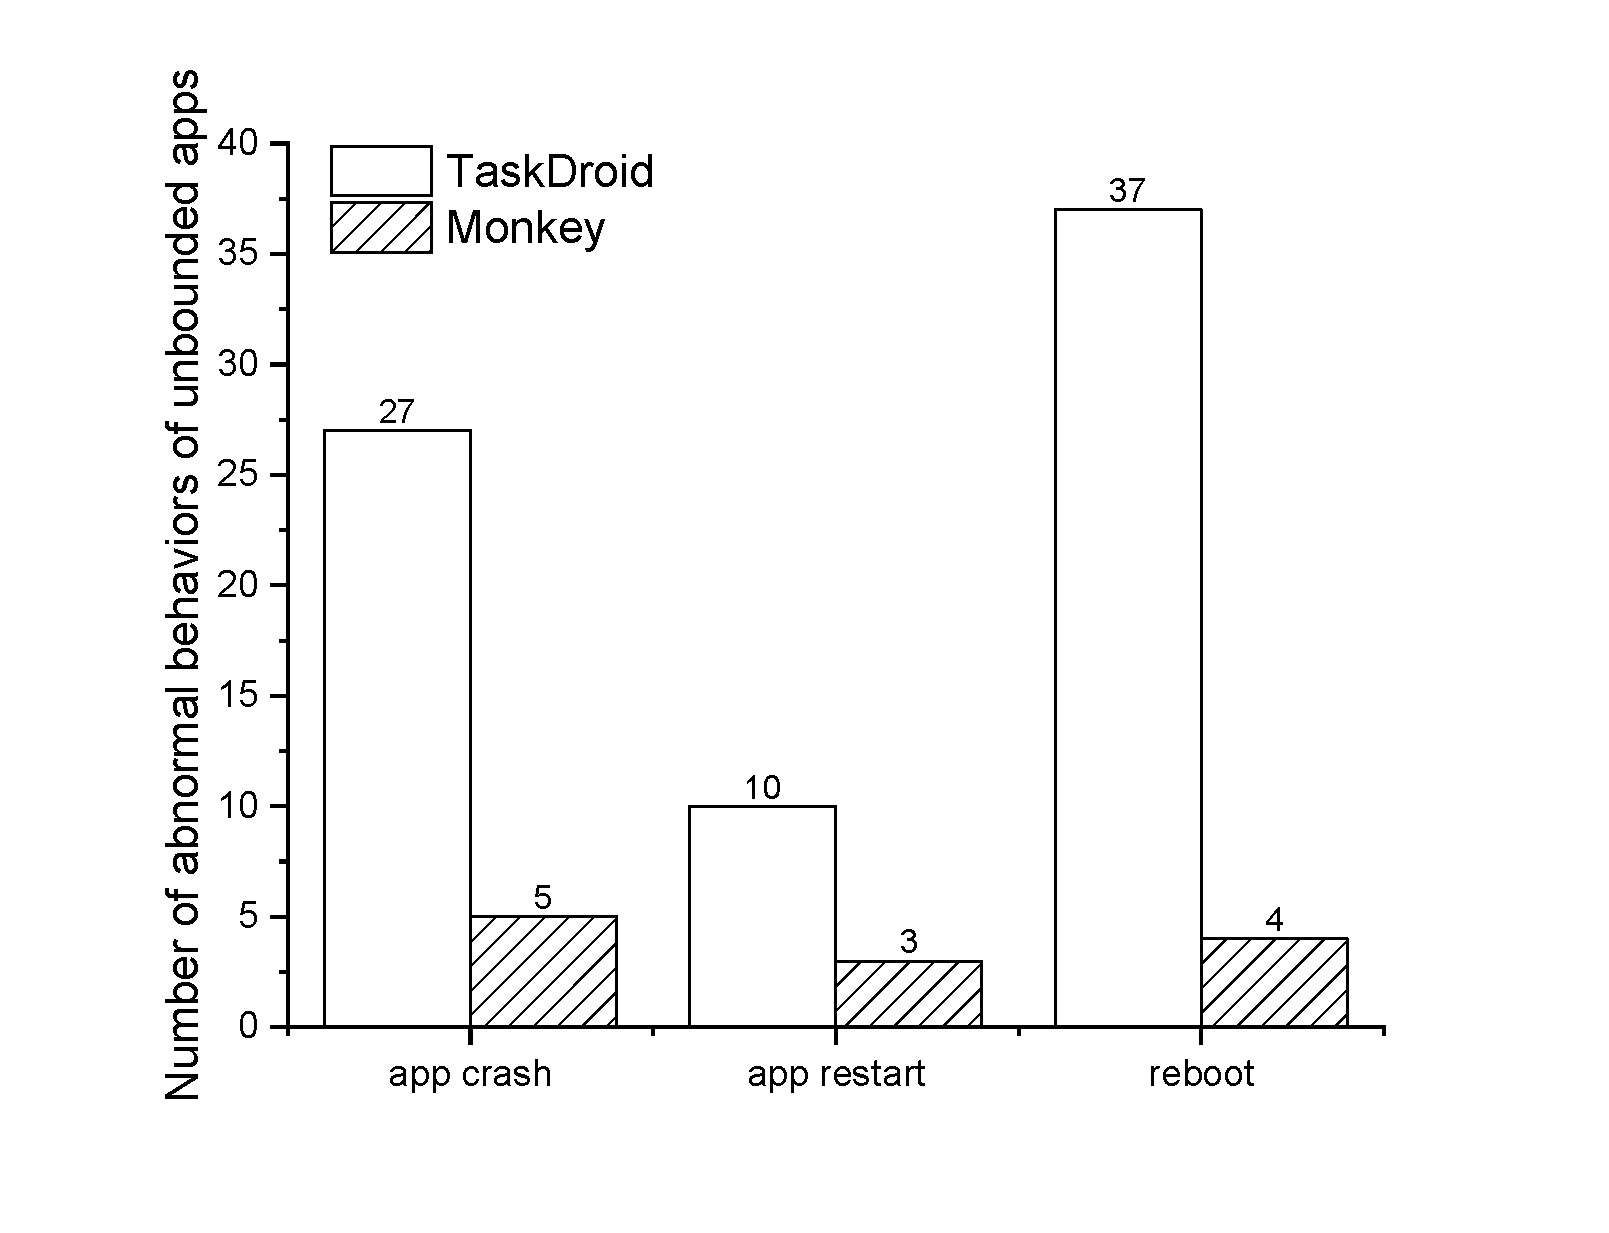
\includegraphics[width=8cm]{cmp-monkey.pdf}
	\caption{\revision{Number of abnormal behaviors of unbounded apps by TaskDroid and Monkey}}
	\label{fig:cmp-monkey}
\end{figure}


%\begin{table*}%[t]
%	\begin{center}   
%		\caption{Threat of unboundedness of popular commercial apps\label{tab:threatpop} }
%		\begin{tabular}{|c|c|c|c|c|c|}   
%			\hline   \textbf{Source} &\begin{tabular}{c}\textbf{unboundedness} \\ \textbf{problem}\end{tabular}&\textbf{Package name} & size(MB) &\begin{tabular}{c} \textbf{\#repetitions of} \\ {\bf the witness cycle}\end{tabular} & \textbf{Abnormal behavior} \\   
%			%
%			\hline   GooglePlay& task  & com.taobao.taobao & 151.0 & 66 & reboot  \\ 
%			\hline   GooglePlay& task  & com.jingdong.app.mall & 92.6 & 59 & reboot  \\ 
%			\hline   GooglePlay& task  & com.amazon.mShop.android.shopping & 73.8 & 73 & reboot  \\ 
%			\hline   GooglePlay& task  & com.contextlogic.wish & 21.9 & 63 & reboot  \\ 
%			\hline   GooglePlay& task  & com.google.android.youtube & 121.3 & 54 & reboot  \\ 
%			\hline   GooglePlay& task  & com.netflix.ninja & 100.6 & 76 & reboot  \\ 
%			\hline   GooglePlay& task  & com.instagram.android & 49.2 & 89 & reboot  \\ 
%			\hline   GooglePlay& task  & com.zhiliaoapp.musically & 167.8 & 65 & reboot  \\ 
%			\hline   GooglePlay& task  & com.facebook.katana & 74.2 & 96 & reboot  \\ 
%			\hline   
%		\end{tabular}   
%	\end{center}   
%\end{table*}

%%%%%%%%%%%%%%%%%%%%%%%%%%%%%%%%%%%%%%%%%%%%%%%%%%%%%%%%%%%%%%%%%%%%%%%%%%%%%%%%%%%%%%%%%%%%%%%%%%%%%%%%%%%%%%%%%%%%%



\subsubsection{Comparison of the impact of different model extractors}\label{sec:cmp}
%
We compare the impact of the following three model extractors on the effectiveness of the task/fragment container unboundedness problems: ICCBot$_{\AMASS}$, ICCBot, and ActExtractor, where ActExtractor is the model extractor from  \cite{HCWWY19}, where only activities were considered while fragments were ignored. 

We first run experiments to compare the capabilities of the three extractors to construct {\AMASS} models. The experiment results are in Figure~\ref{fig:cmp-extractor-model}, which include the numbers of models constructed by these extractors and the average number of transition rules in these models. From Figure~\ref{fig:cmp-extractor-model}, we can see that ICCBot$_{\AMASS}$ constructs more models than the other two extractors, since it is the only extractor that is able to construct models dynamically from APK files. Moreover, the average number of transition rules in the models constructed by ICCBot$_{\AMASS}$ is greater than the other two extractors, which is mainly because the models constructed dynamically by ICCBot$_{\AMASS}$ include much more transition rules than those constructed statically, since these apps are the ones that cannot be decompiled and normally large %popular 
commercial apps. 

\begin{figure}[htbp]
	\begin{minipage}[t]{0.49\linewidth}
		\centering
		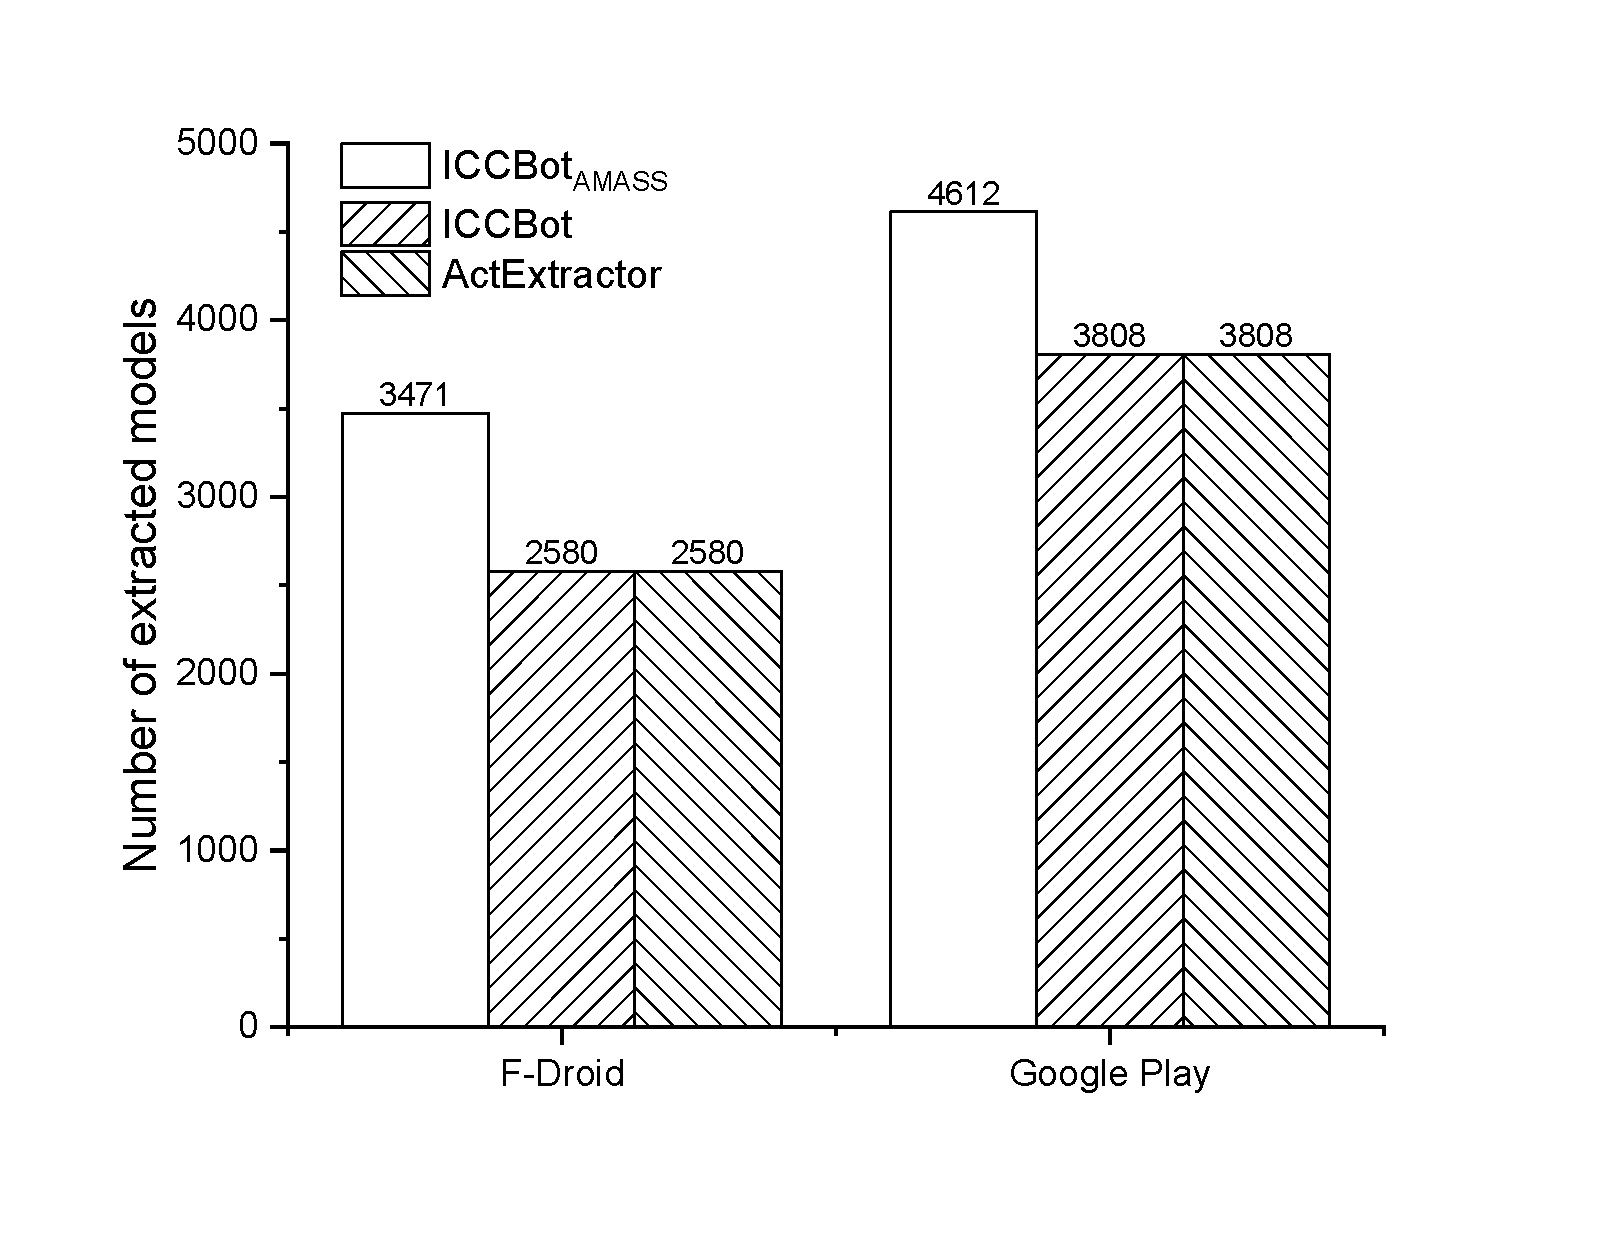
\includegraphics[width=3.2in]{model.pdf}
	\end{minipage}
	\begin{minipage}[t]{0.49\linewidth}
		\centering
		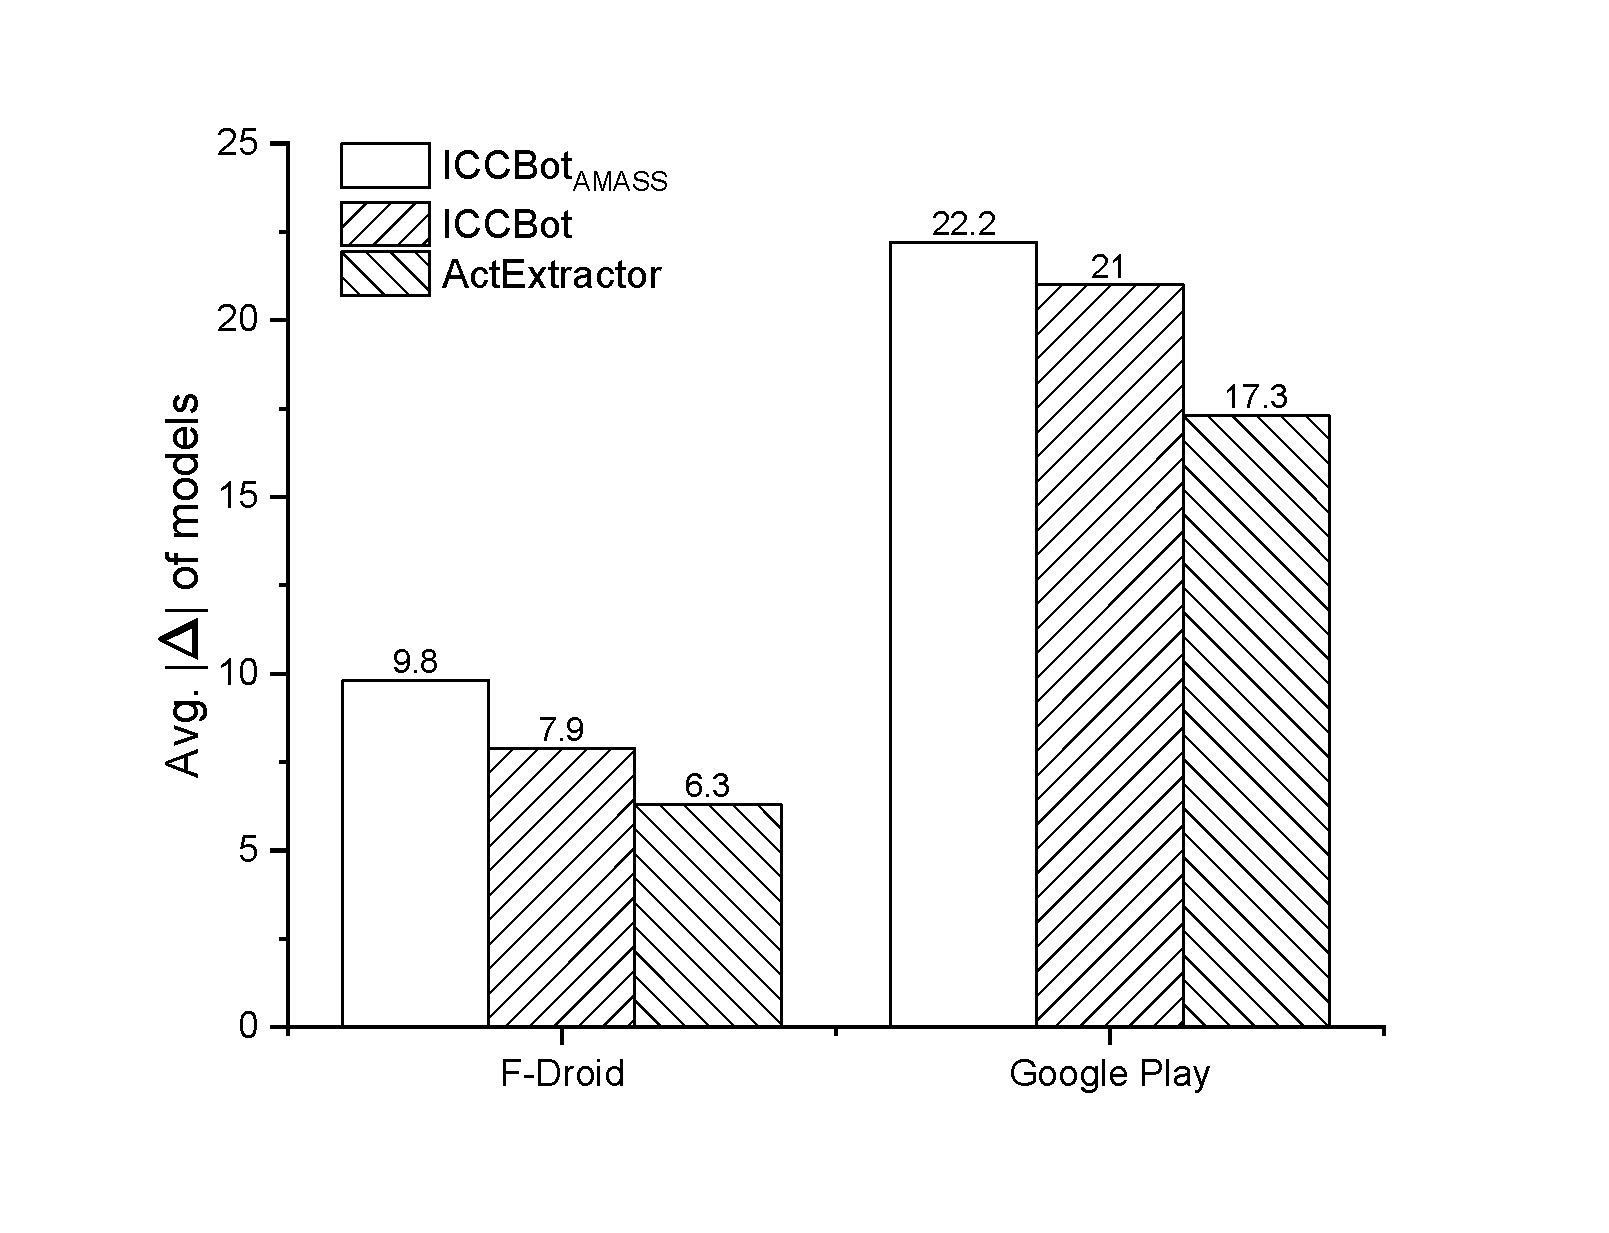
\includegraphics[width=3.2in]{delta.pdf}
	\end{minipage}
	\caption{Numbers of models extracted by different extractors and the average number of transitions in these models}
	\label{fig:cmp-extractor-model}
\end{figure}

%In this section, we conduct a comparison of model extraction and unboundedness using different {\AMASS} extractors, namely ICCBot$_{\AMASS}$, Extractor$_{\mathsf{APLAS}}$, and ICCBot. It is worth noting that Extractor$_{\mathsf{APLAS}}$ is the extractor utilized in \cite{HCWWY19}, which exclusively focuses on extracting activity transitions.

%Based on the observations from Figure~\ref{fig:cmp-extractor-model}, it is evident that ICCBot$_{\AMASS}$ exhibits the highest number of extracted models for both F-Droid apps and %Google Play apps, while the other two extractors yield the same results.
%The superior performance of ICCBot$_{\AMASS}$ can be attributed to its capability of extracting more models using dynamic {\sf AMASSExtractor}, which is not feasible with the other two extractors.
%Regarding the average size of transition rules in the extracted models, ICCBot$_{\AMASS}$ surpasses both ICCBot and Extractor$_{\mathsf{APLAS}}$. This can be attributed to the fact that ICCBot$_{\AMASS}$ and ICCBot are capable of extracting fragment transitions, while Extractor$_{\mathsf{APLAS}}$ lacks this functionality, and for the models extracted by the dynamic extractor, the average size of transition rules is greater than those extracted by the static extractor.

\begin{figure}[htbp]
	\begin{minipage}[t]{0.49\linewidth}
		\centering
		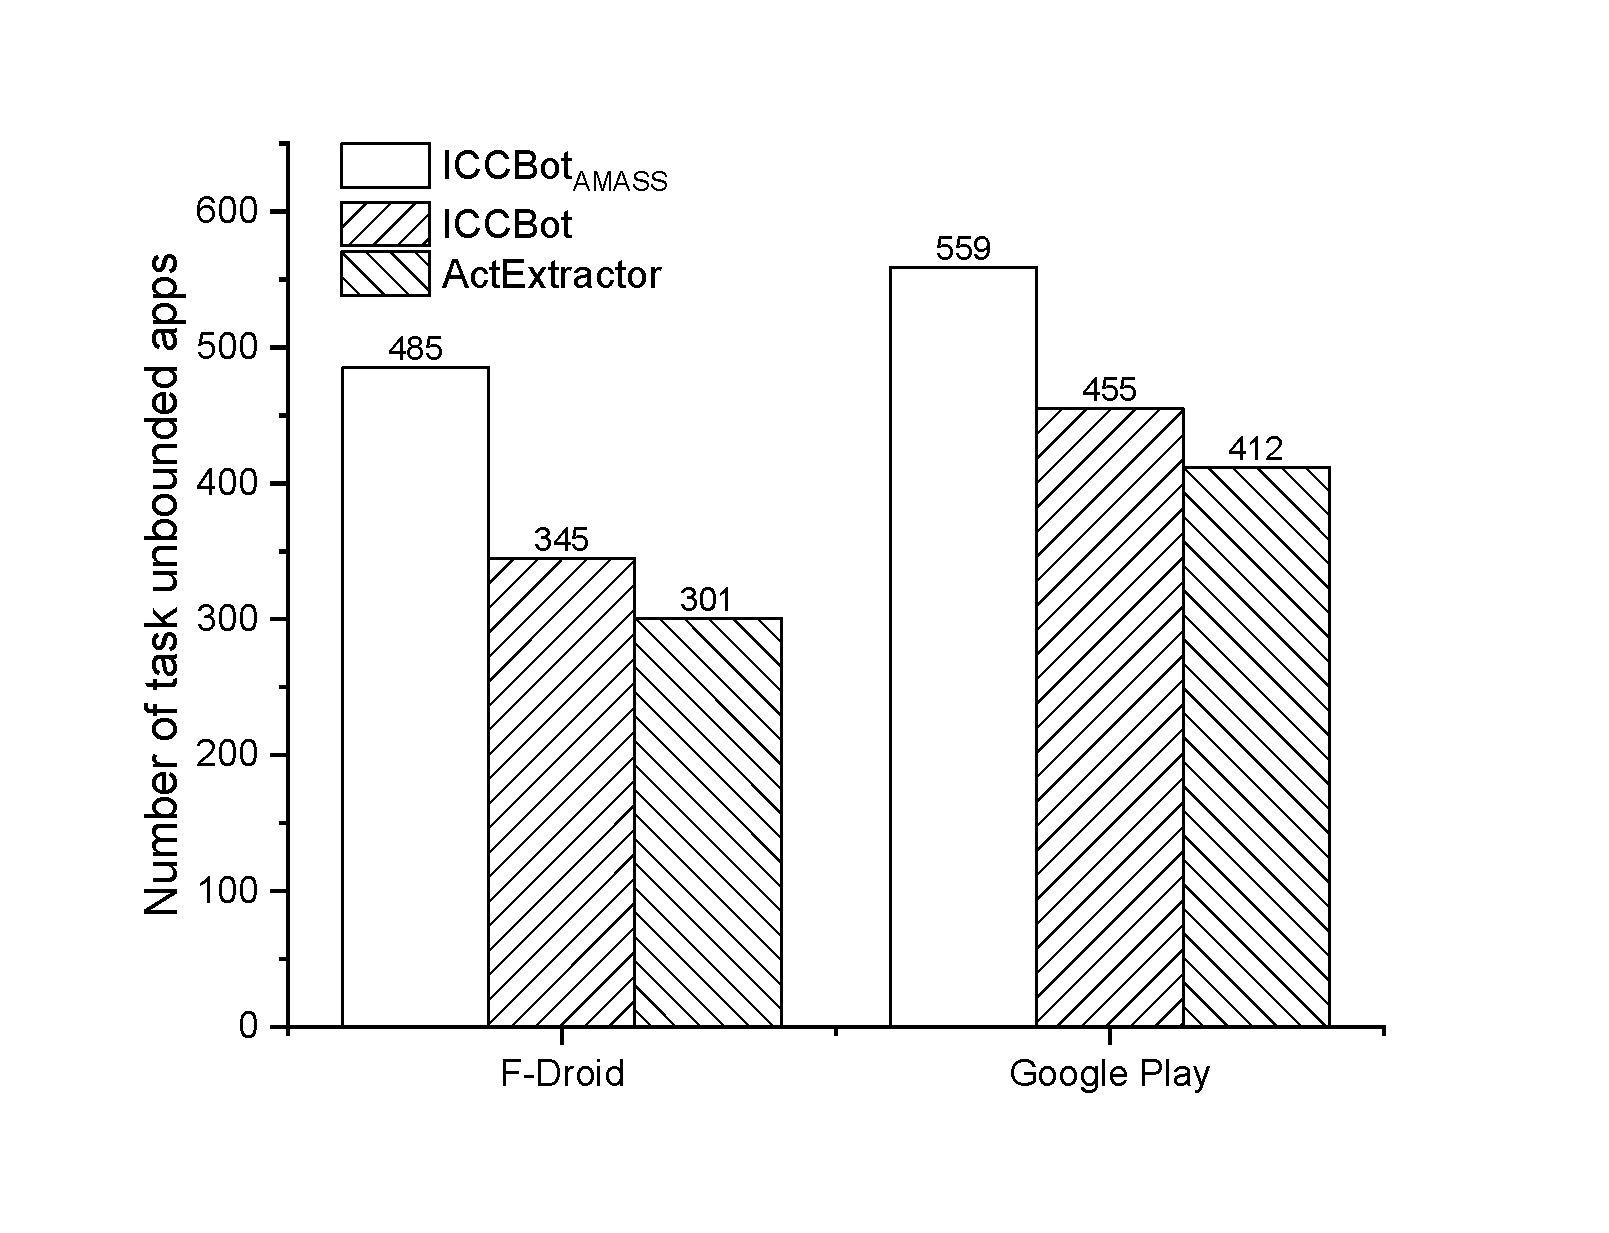
\includegraphics[width=3.2in]{task_ubd.pdf}
	\end{minipage}
	\begin{minipage}[t]{0.49\linewidth}
		\centering
		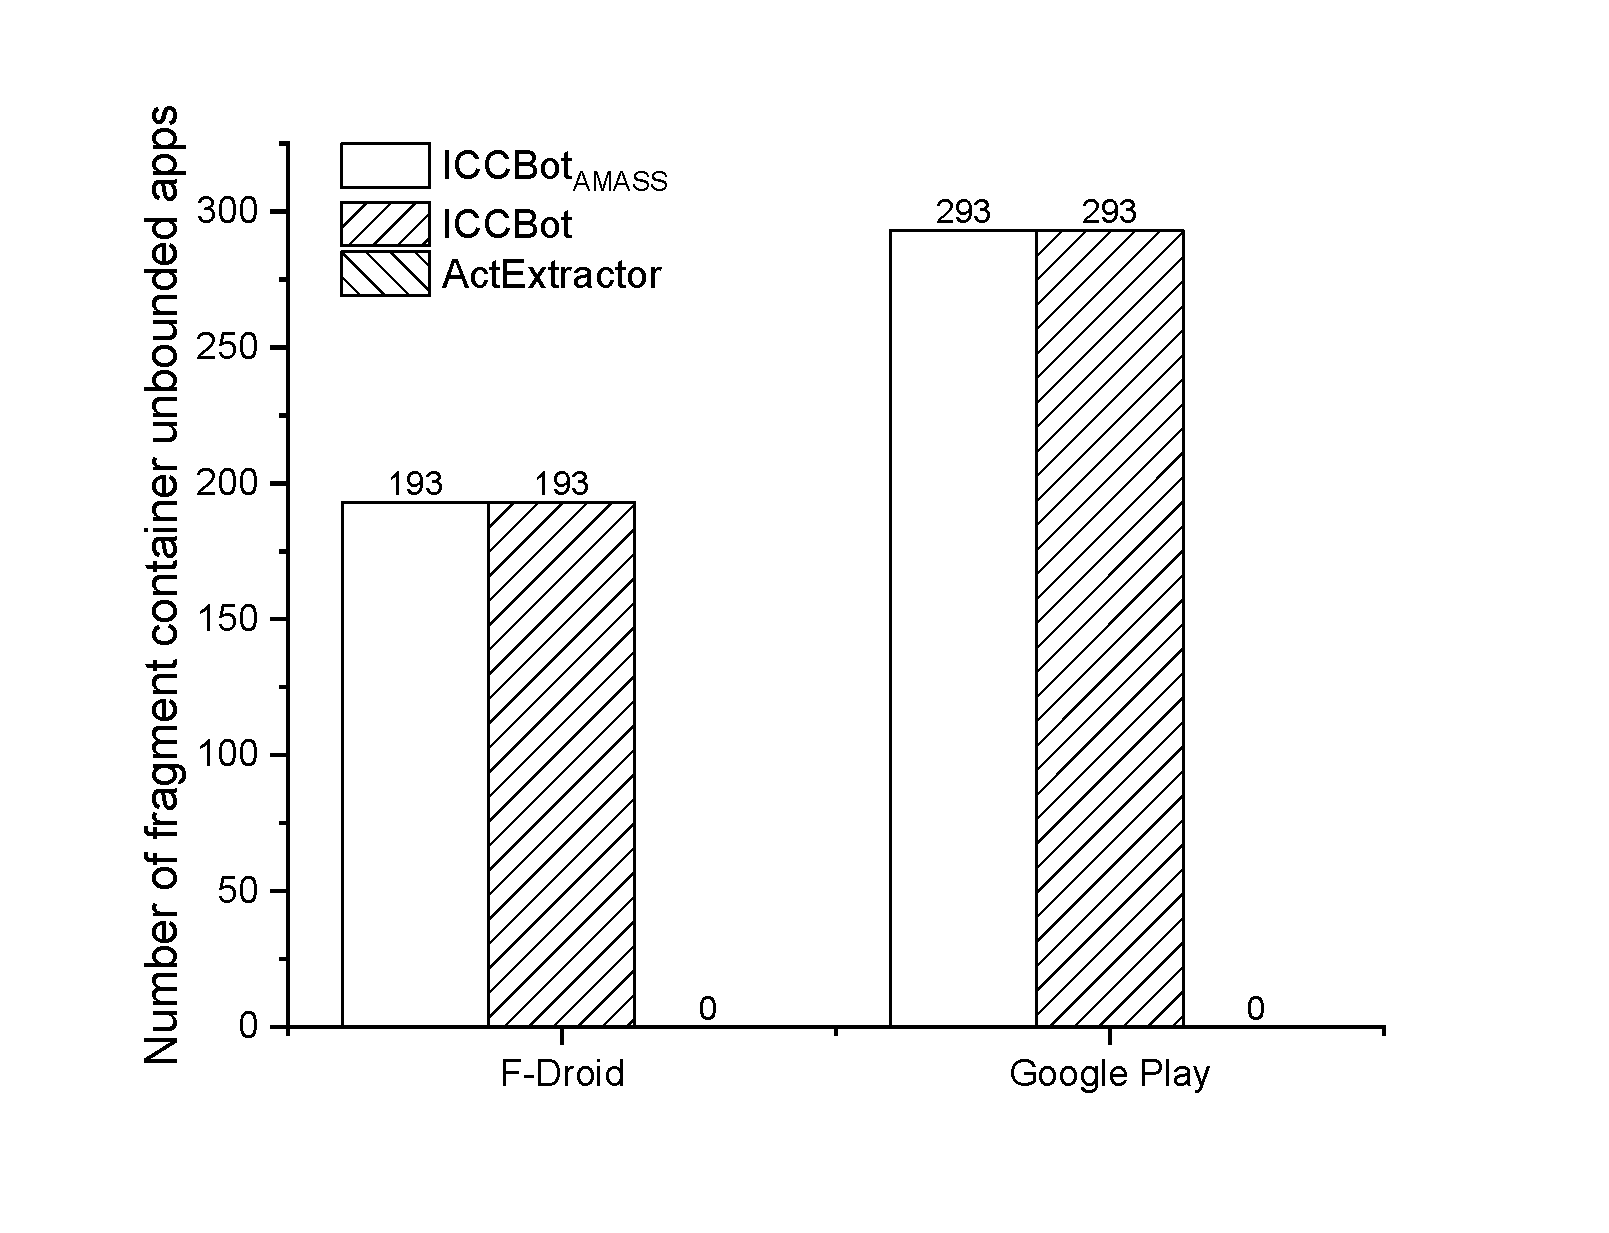
\includegraphics[width=3.2in]{frag_ubd.pdf}
	\end{minipage}
	\caption{Numbers of task/fragment container unbounded apps using different extractors}
	\label{fig:cmp-extractor-ubd}
\end{figure}


To compare the impact of different extractors on TaskDroid, for each app, we run {\sf AMASSAnalyzer} on the three models constructed by the three extractors for the app. We summarize the results in Figure~\ref{fig:cmp-extractor-ubd}. From Figure~\ref{fig:cmp-extractor-ubd}, we can see that the number of task unbounded apps is the greatest when ICCBot$_{\AMASS}$ is used. \revision{This is due to the fact that ICCBot$_{\AMASS}$ extracts more models than the other two extractors since it utilizes the dynamic approach to extract the models from the commercial apps that cannot be decompiled. In Table~\ref{tab:threatpop}, by repeatedly executing the witness cycles, we confirm that among these apps whose models are constructed dynamically by ICCBot$_{\AMASS}$, 9 apps are indeed task unbounded. Note that ICCBot and ActExtractor are unable to construct models from these apps since their APK files cannot be decompiled successfully by Soot. }
On the other hand, TaskDroid reports the same number of fragment container unbounded apps for ICCBot$_{\AMASS}$ and ICCBot. This is due to the fact that although ICCBot$_{\AMASS}$ extracts more information about fragments than ICCBot, e.g., the API addToBackstack(TS), these information has no impact on our static analysis algorithm for the fragment container unboundedness problem (see Section~\ref{sec:static}). Moreover, no fragment unboundedness is reported for the models extracted by ActExtractor, since it only extracts the information for activities. 
%\jinlong{In conclusion, compared with \cite{HCWWY19}, TaskDroid detects more task unbounded apps and analyzes fragment container unbounded problem which \cite{HCWWY19} does not consider.}

%Based on Figure~\ref{fig:cmp-extractor-ubd}, it can be observed that ICCBot$_{\AMASS}$ exhibits the highest number of extracted models and the average size of transition rules. Consequently, ICCBot$_{\AMASS}$ detects a larger number of task unbounded apps compared to the other two extractors.  The discrepancy in the number of task unbounded apps detected between ICCBot and Extractor$_{\mathsf{APLAS}}$ can be attributed to the inability of Extractor$_{\mathsf{APLAS}}$ to extract fragment transitions. As a result, there are fewer transitions between activities, resulting in a lower number of task unbounded apps detected by Extractor$_{\mathsf{APLAS}}$ compared to ICCBot. 
%Regarding the number of fragment container unbounded apps detected, both ICCBot$_{\AMASS}$ and ICCBot yield the same results, as the dynamic {\sf AMASSExtractor} is unable to extract fragment transitions. However, Extractor$_{\mathsf{APLAS}}$ lacks the capability to extract fragment transitions, resulting in zero detections of fragment container unbounded apps by Extractor$_{\mathsf{APLAS}}$.


% \subsubsection{\revision{}}\label{sec:cross-app}
%%%%%%%%%%%%%%%%%%%%%%%%%%%%%%%%%%%%%%%%%%%%%%%%%%%%%%%%%%%%%%%%%%%%%%%%%%%%%%%%%%%%%%%%%%%%%%%%%%%%%%

\subsection{Validation of the  ``small number of tasks''  and ``small height of stacks''  hypotheses} \label{sec:hyp}

We validate the ``small number of tasks''  and ``small height of stacks''  hypotheses used in Section~\ref{sec:static}.
%
Recall that for the analysis of task unboundedness in Section~\ref{sec:static},  we hypothesize that only a small number $k$ of tasks are involved. 

We first evaluate the validity of the ``small number of tasks'' hypothesis for task unboundedness by varying  $k$ from $0$ to $3$ and checking the growth of the number of task unbounded apps detected by {\tool}. 
The experimental results are shown in Figure~\ref{fig:k}.
We observe that when $k$ is increased from $1$ to $2$, the number of task-unbounded apps increases only slightly.
Moreover, when $k$ is increased from $2$ to $3$, the number of task-unbounded apps keeps unchanged.
This suggests that, in order to identify those task-unbounded apps, a small $k$ suffices (in this case $k=2$). This also justifies our choice of $k$ in the static analysis of task unboundedness for {\AMASS} models.  This phenomenon is explained by the observation that for a majority of apps, %satisfy that 
the number of task affinities of their activities is small (or even equal to 1).
%
% \begin{figure}%[h]
% \centering
% 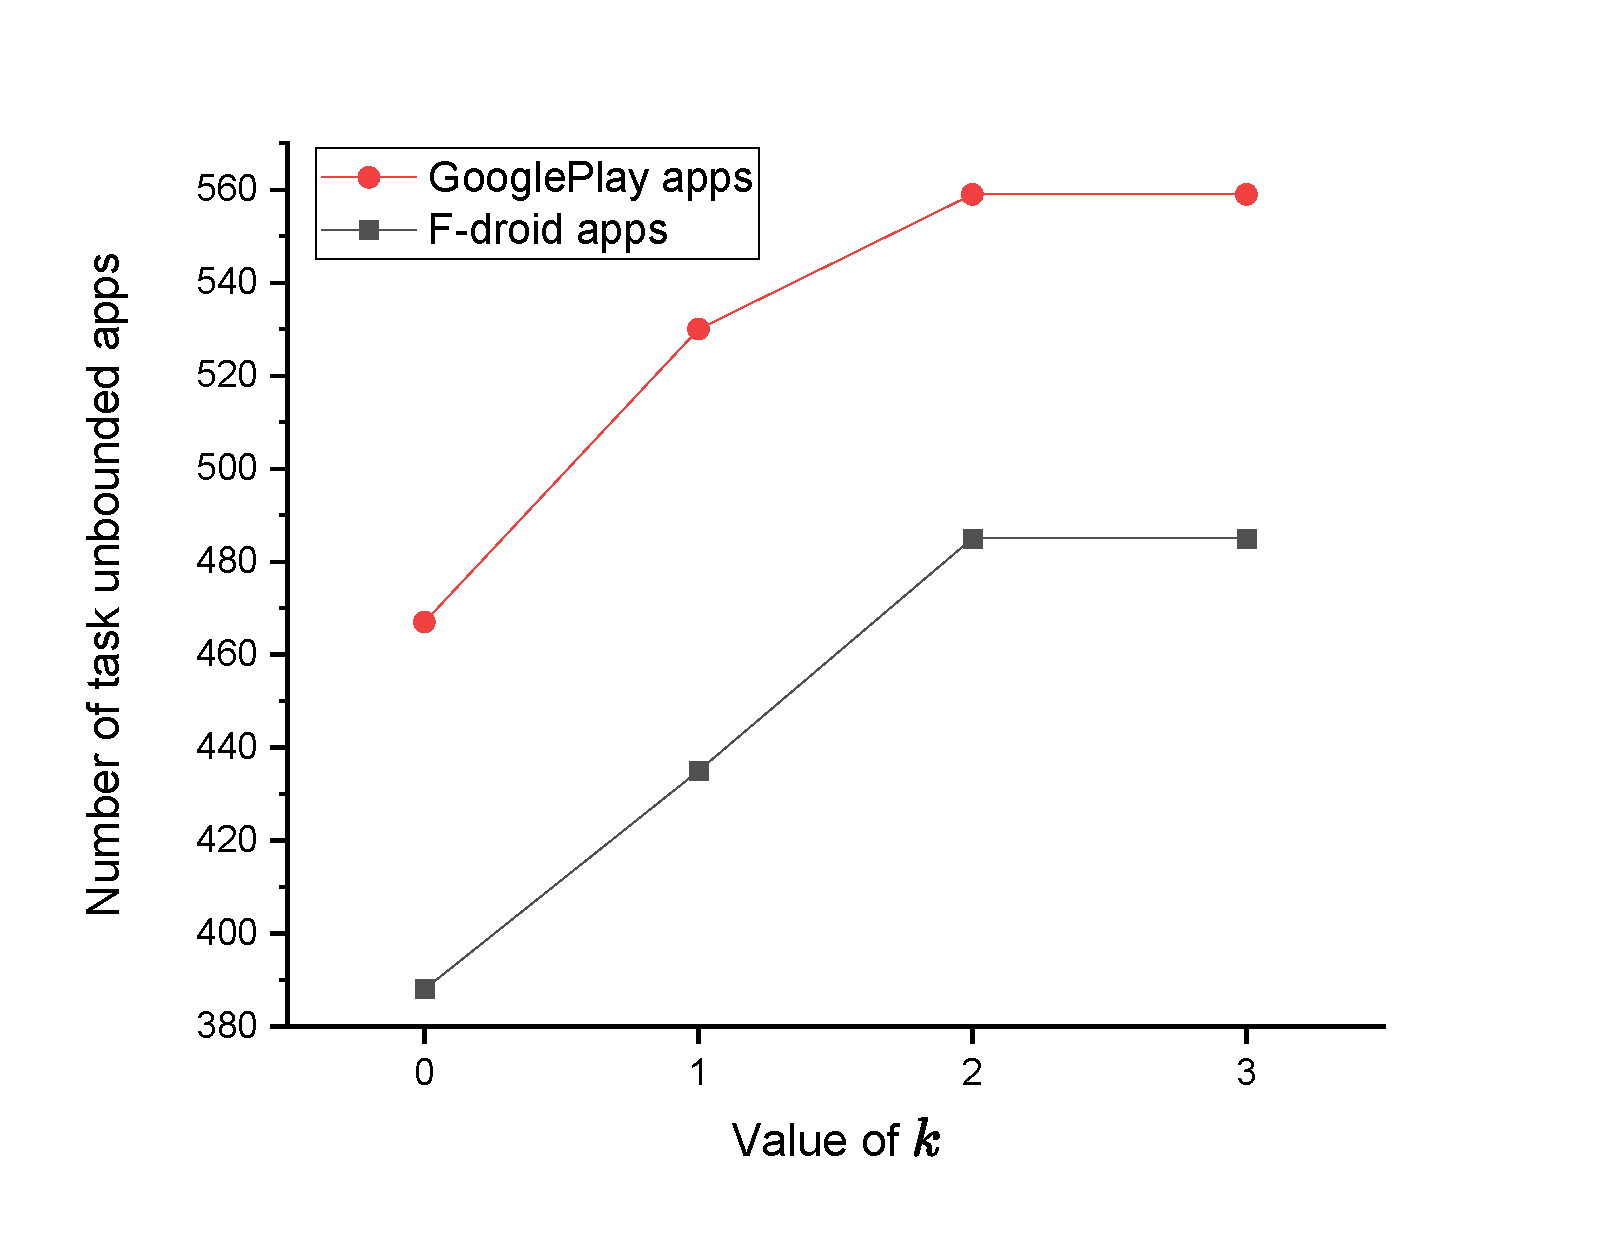
\includegraphics[scale=0.4]{k.pdf}
% \caption{Small number hypothesis: k}
% \label{fig:k}
% \end{figure}

Moreover, in Section~\ref{sec:static}, the height bound $\hbar = 6$ of stacks was used to generate the witnessing transition sequences for task unbounded and fragment container unbounded {\AMASS} models. We then carry out experiments to validate this ``small height of stacks'' hypothesis. 
The experiments proceed as follows: we first set $\hbar = 1$, use {\nuxmv} to generate the witnessing transition sequences for the  {\AMASS} models that are identified as ``task unbounded''  by TaskDroid, and count the number of models for which the witnessing transition sequences can be successfully generated. Then we experiment $\hbar=2$--$7$. % and do the same thing as for $\hbar = 2$. 
The results are summarized in Figure~\ref{fig-small-height}, where we can see that the number of models for which the witnessing transition sequences can be successfully generated grow when $\hbar$ is increased from $1$ to $6$, while keep unchanged when $\hbar$ is increased from $6$ to $7$. The results justify the ``small height of stacks'' hypothesis and our choice of $\hbar = 6$ in Section~\ref{sec:static}. 


%Recall that for the reachability analysis we hypothesize that the heights of involved tasks are bounded by a small number $\hbar$. Likewise, for the task boundedness analysis,  we hypothesize that only a small number $k$ of tasks are involved. In our experiments, we indeed set $\hbar$ to $4$ and $k$ to 2. In this section, we  aim to investigate whether these hypotheses are tenable. 
\begin{figure}[htbp]
\centering
\begin{minipage}[t]{0.48\textwidth}
\centering
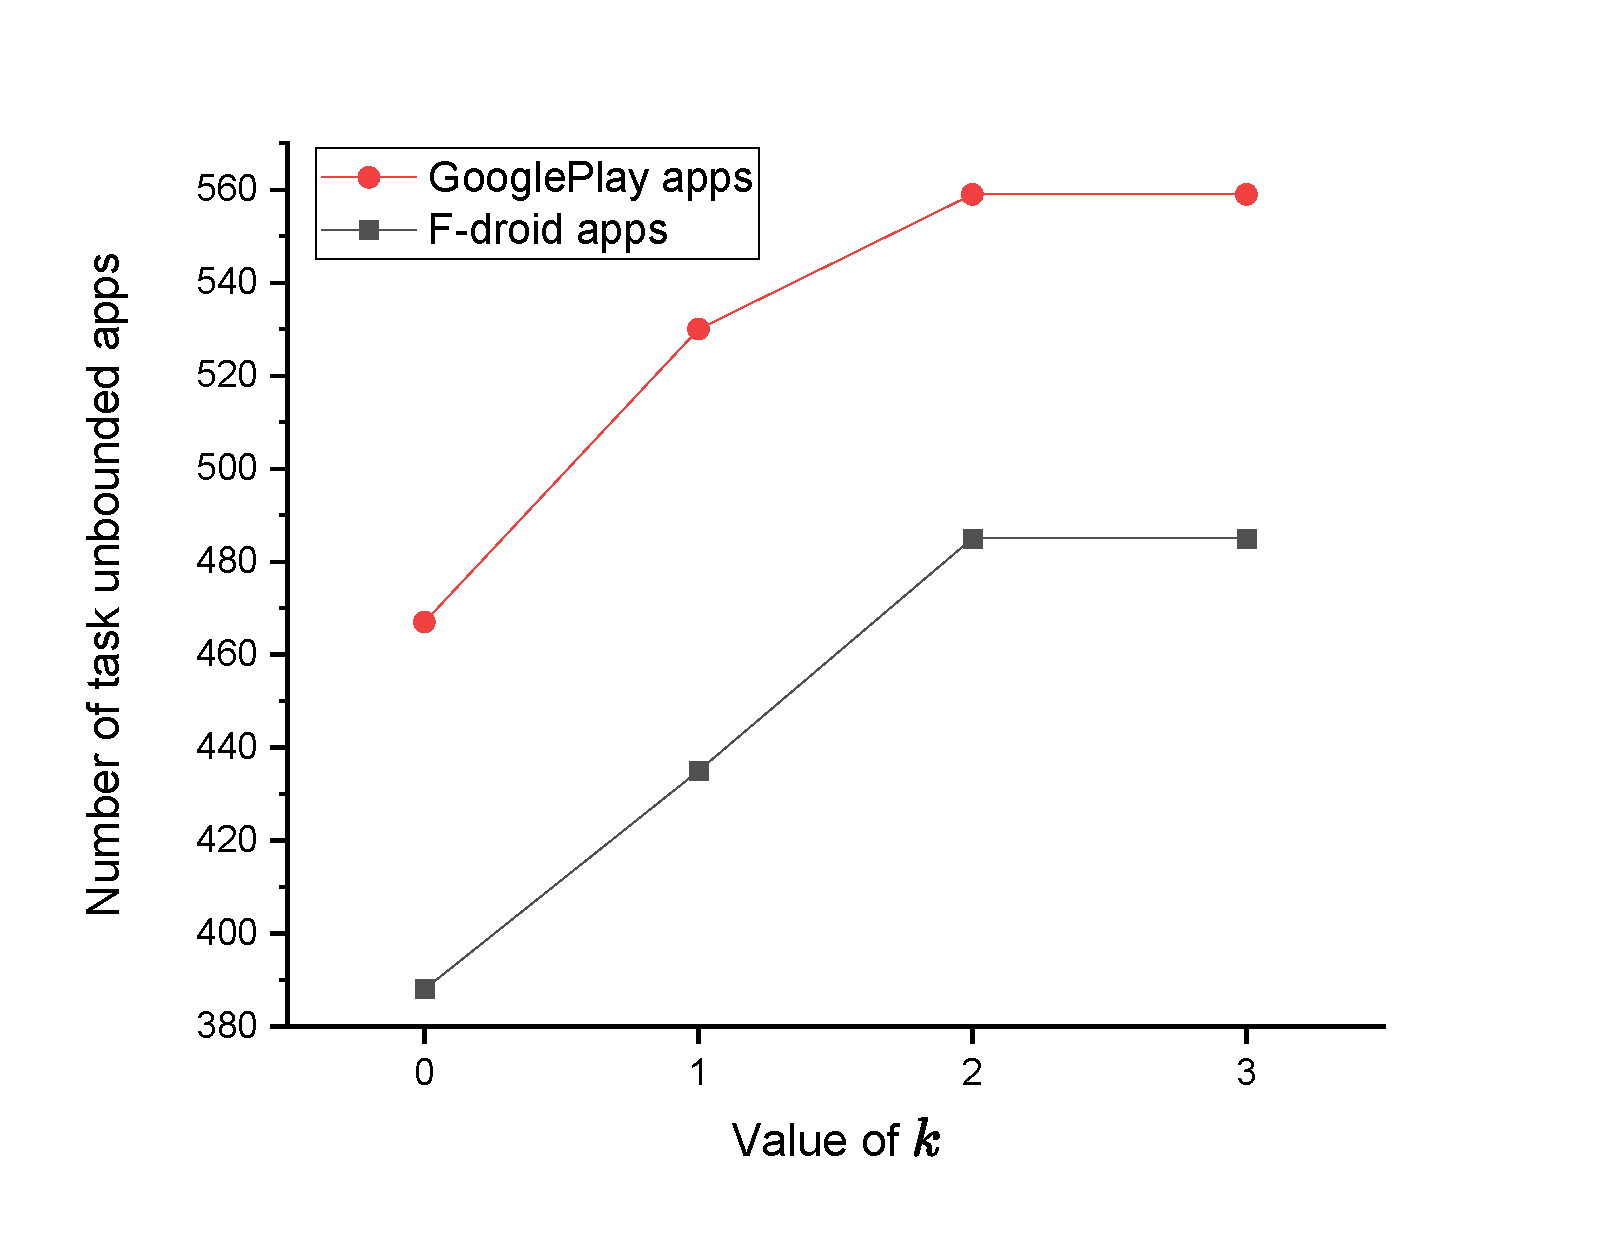
\includegraphics[width=8cm]{k.pdf}
\caption{``Small number of tasks'' hypothesis: $k$}
\label{fig:k}
\end{minipage}
\begin{minipage}[t]{0.48\textwidth}
\centering
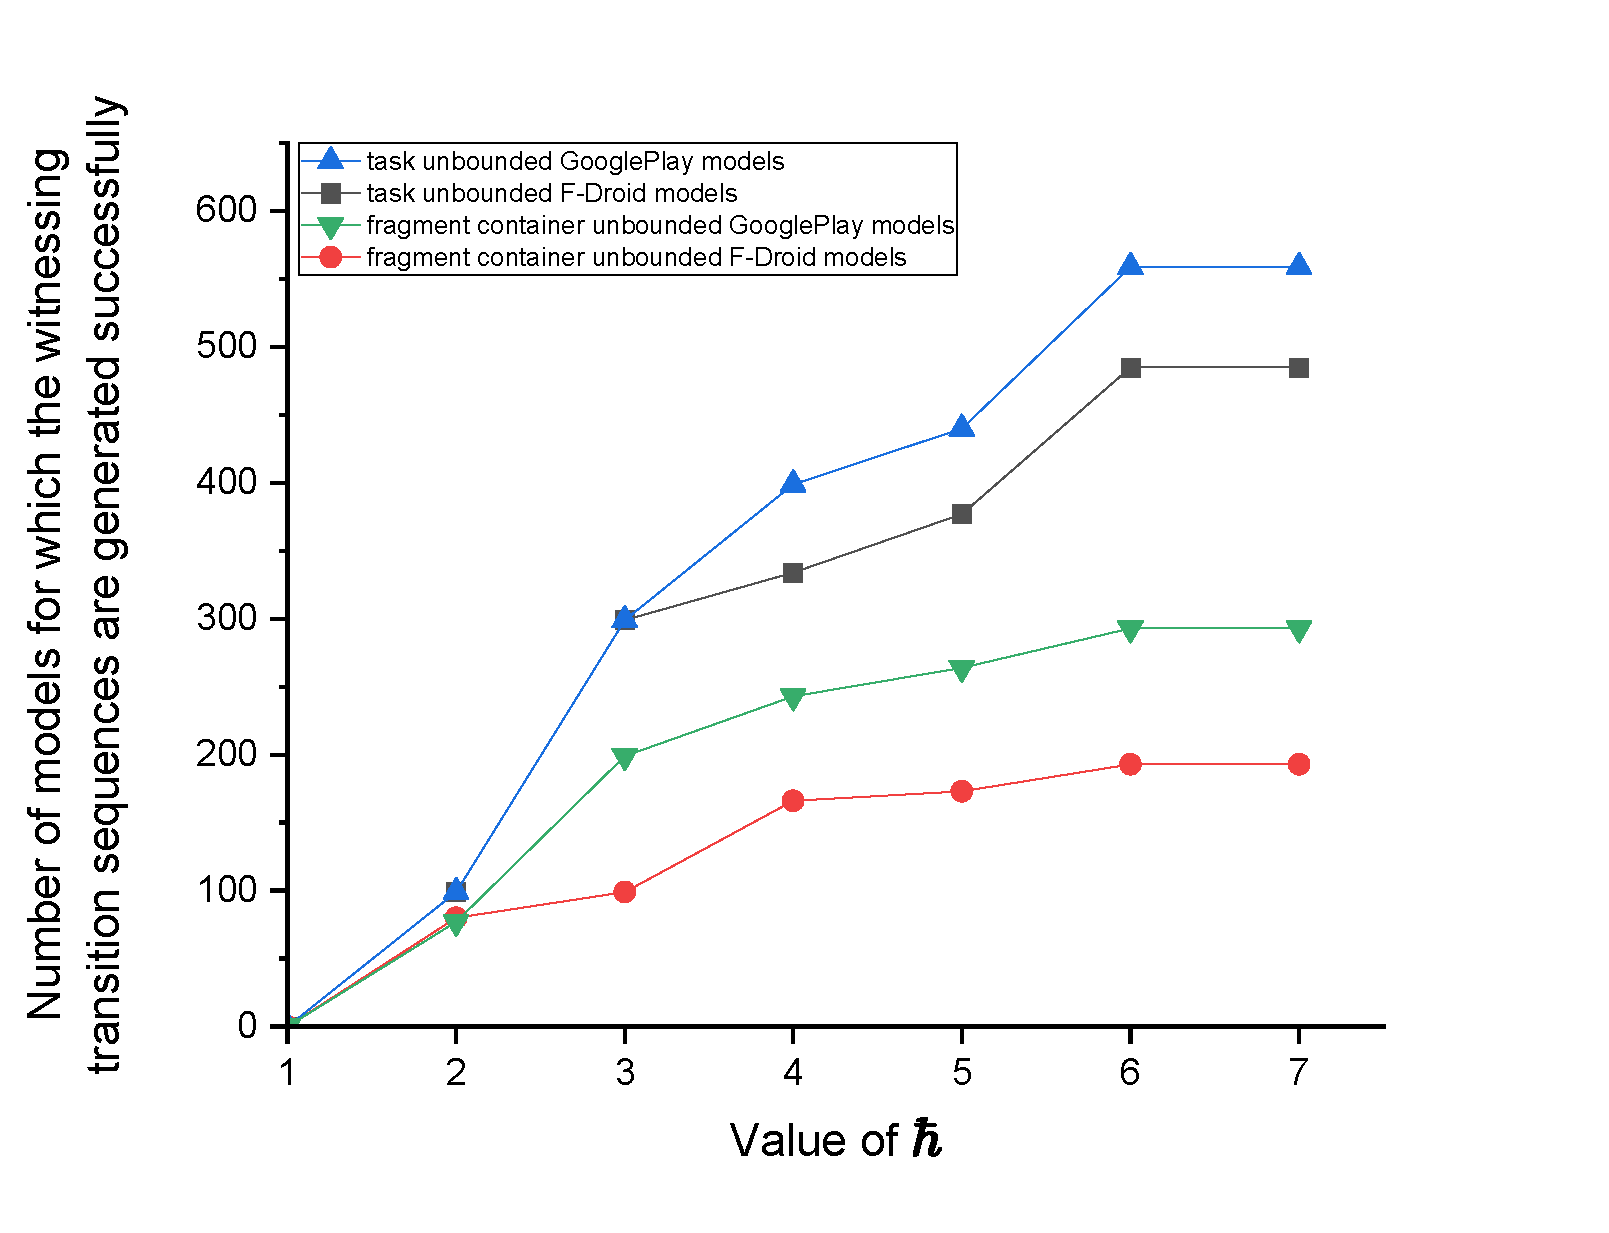
\includegraphics[width=8cm]{h.pdf}
\caption{``Small height of stacks'' hypothesis: $\hbar$}
\label{fig-small-height}
\end{minipage}
\end{figure}
	
% \begin{figure}%[h]
% \centering
% 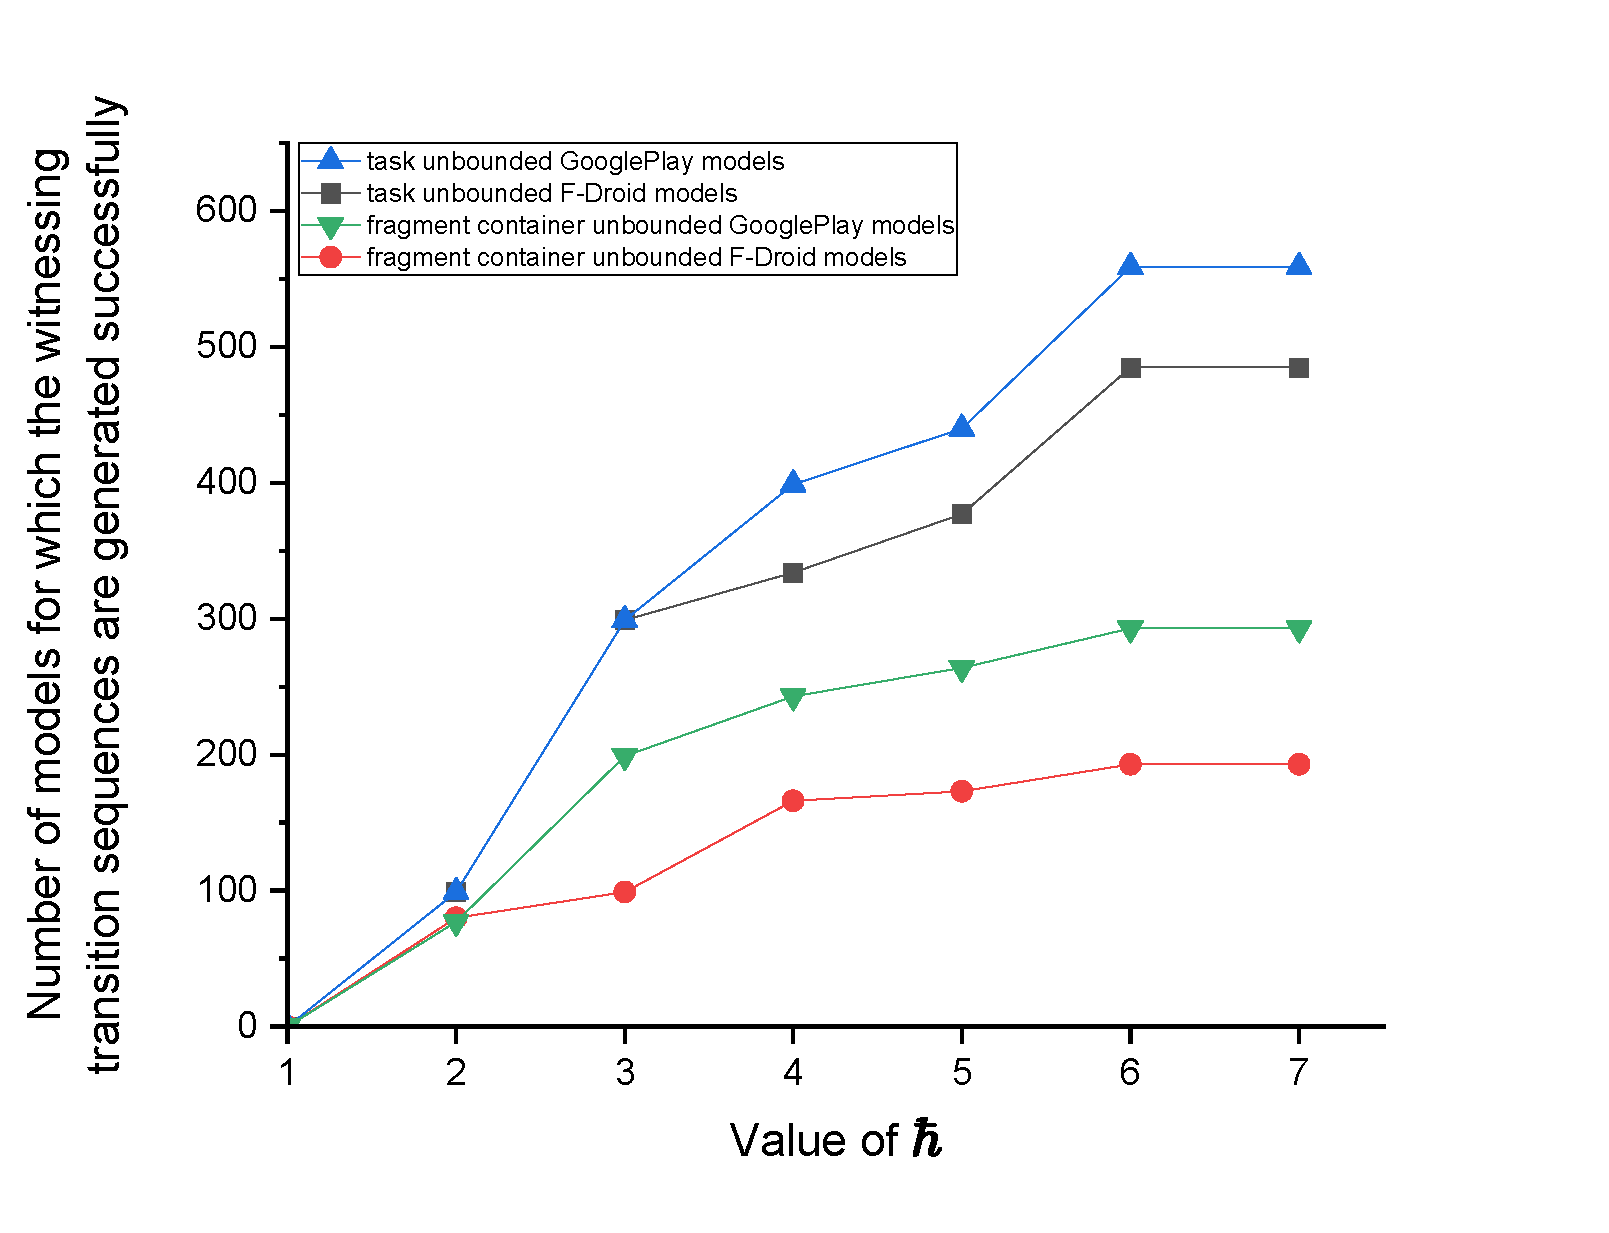
\includegraphics[scale=0.45]{h.pdf}
% \caption{``Small  height of stacks'' hypothesis}
% \label{fig-small-height}
% \end{figure}


%the number $k$ has little influence 
% obtain the conclusion that $k$ has little influence on the results, hence a small number $k$ can lead almost correct results. There are two reasons leading this conclusion, 1) there are nearly $90\%$ apps have only one single affinity in our bench mark, hence $k = 0$ can solve almost all of them. 2) there are nearly $70\%$ apps are acyclic which can lead to be stack bounded directly.



%the size means the average back pattern size of an activity in the bench mark, and 
%$k$ is the maximal stack height for each app. $\Delta_{size}$ means the difference of back pattern size of the same activity in the same app between the different value of $k$. Hence we can obtain the conclusion that there are little difference between $k = 4$ and $k = 6$, this is because the maximal stack height in most apps are not very large.

%Based on these results, we conclude that $\hbar$-reachability and $k$-task boundedness  provide sufficiently precise analysis results for reasonably small $\hbar$ or $k$.    

%We carry  out all experiments on a Linux server with a CPU of Intel\textsuperscript{\textregistered} Xeon\textsuperscript{\textregistered} Processor E5-2680 v4 at 2.40GHz and 64GB memory.

 

\hide{
\begin{table}%[htb]   
\begin{center}   
\begin{tabular}{|c|c|c|c|}   
    \hline   \textbf{Source} &\textbf{Extractor}  &\begin{tabular}{c}\textbf{\#Unbounded}\\ \textbf{models}\end{tabular} & \begin{tabular}{c} \#\textbf{witness cycles} \\ \textbf{per model}\end{tabular}  \\   
	\hline
    \multirow{3}{*}{F-Droid} &ICCBot$_{\AMASS}$ & 485/3,471(14.0\%) & 3.3\\
    \cline{2-4}    
     &ICCBot$_{\mhcancel{\frag}}$ & 416/3,471(12.0\%) & 3.1\\
    \cline{2-4}    
     &ICCBot & 332/2,580(12.9\%) & 3.0\\
	\hline
    \multirow{3}{*}{Google Play} &ICCBot$_{\AMASS}$& 559/4,612(12.1\%)&3.9\\
    \cline{2-4}    
     &ICCBot$_{\mhcancel{\frag}}$ & 512/4,612(11.1\%)&3.6\\
    \cline{2-4}    
     &ICCBot & 382/3,808(10.0\%)&3.4\\
\hline   
\end{tabular}   
\caption{Task Unboundedness under different extractors \label{tab:taskbound-model} }
\end{center}   
\end{table}

\begin{table}%[htb]   
\begin{center}   
\begin{tabular}{|c|c|c|c|}   
    \hline   \textbf{Source} &\textbf{Extractor}  &\begin{tabular}{c}\textbf{\#Unbounded}\\ \textbf{models}\end{tabular} & \begin{tabular}{c} \#\textbf{witness cycles} \\ \textbf{per model}\end{tabular}  \\   
	\hline
    \multirow{3}{*}{F-Droid} &ICCBot$_{\AMASS}$ & 193/2,580(7.5\%) & 2.5\\
    \cline{2-4}    
     &ICCBot$_{\mhcancel{\frag}}$ & 0/2,580(0\%) & 0\\
    \cline{2-4}    
     &ICCBot & 193/2,580(7.5\%) & 2.5\\
	\hline
    \multirow{3}{*}{Google Play} &ICCBot$_{\AMASS}$& 293/3,808(7.7\%)&3.0\\
    \cline{2-4}    
     &ICCBot$_{\mhcancel{\frag}}$ & 0/3,808(0\%)&0\\
    \cline{2-4}    
     &ICCBot & 293/3,808(7.7\%)&3.0\\
\hline   
\end{tabular}   
\caption{Fragment Container Unboundedness under different extractors \label{tab:fragbound-model} }
\end{center}   
\end{table}
}

\hide{
\begin{table}%[htb]   
\begin{center}   
\begin{tabular}{|c|c|c|c|c|c|}   
    \hline   \textbf{Source} & \textbf{Unbounded} & \textbf{Android 6.0} & \textbf{Android 7.0}  & \textbf{Android 8.0-10.0} &\textbf{Android 11.0-13.0} \\   
    \hline   \multirow{2}{*}{F-Droid} & Task & 490 & 484 & 486 & 485 \\
    \cline{2-6}    & Fragment Container & 193 & 193 & 193 & 193\\
    \hline \multirow{2}{*}{Google Play} & Task & 568 & 555 & 562 & 559 \\
    \cline{2-6}    & Fragment Container & 293 & 293 & 293 & 293 \\
\hline   
\end{tabular}   
\caption{\revision{Unboundedness under different Android versions \label{tab:bound} }}
\end{center}   
\end{table}
}

\hide{
\begin{table}%[htb]   
\begin{center}   
\begin{tabular}{|c |c |c |c |c |c |c |c|c|}   
    \hline    
    \multirow{2}{*}{\textbf{Source}} & \multirow{2}{*}{\textbf{Extractor}}  &\multicolumn{3}{c|}{\textbf{Avg/Max. size of models}} & \multirow{2}{*}{\textbf{\# extracted  models}} \\   
    \cline{3-5}    
    && $|\act|$& $|\frag|$ & $|\Delta|$ &   \\ 
    \hline   
    \multirow{3}{*}{F-Droid} &ICCBot$_{\AMASS}$ &  5.2/70& 0.4/16 & 9.8/475 &  3,471  \\ 
    \cline{2-6}    
     &ICCBot$_{\mhcancel{\frag}}$ &  5.2/70& 0/0 & 6.3/332 &  3,471  \\ 
    \cline{2-6}    
     &ICCBot &  4.9/70& 0.5/16 & 6.9/369 &  2,580  \\ 
    \hline   
    \multirow{3}{*}{Google Play}&ICCBot$_{\AMASS}$  & 7.8/509&0.8/121&22.2/1,956 & 4,612  \\  
    \cline{2-6}    
     &ICCBot$_{\mhcancel{\frag}}$ & 7.8/509&0/0&17.3/1,234 & 4,612  \\  
    \cline{2-6}    
     &ICCBot  & 7.1/509&1.0/121&18.9/1,557 & 3,808  \\  
    % \hline   
    % \multirow{2}{*}{ICCBot} &F-Droid &  3.6/70& 0.4/16 & 5.9/369 &  2,580  \\ 
    % \cline{2-6}    
    %  &Google Play  & 7.1/509&1.0/121&21.0/1956 & 3,808  \\  
\hline   
\end{tabular}   
\caption{Comparison with AMASSExtractors \label{tab:extractor} }
\end{center}   
\end{table}
}
